\documentclass{sig-alternate}

% UTF8 support
\usepackage[utf8x]{inputenc}

\usepackage{subfig}
\usepackage{hyperref}
\usepackage{graphicx}
\graphicspath{{figures/}}
\usepackage{multirow}

\newcommand{\eg}{{\textit{e.g.~}}}
\newcommand{\etal}{{\textit{et al.~}}}
\newcommand{\ie}{{\textit{i.e.~}}}



%
% --- Author Metadata here ---
\conferenceinfo{10th ACM/IEEE International Conference on Human-Robot Interaction}{2015 Portland, USA}
%\CopyrightYear{2007} % Allows default copyright year (20XX) to be over-ridden - IF NEED BE.
%\crdata{0-12345-67-8/90/01}  % Allows default copyright data (0-89791-88-6/97/05) to be over-ridden - IF NEED BE.
% --- End of Author Metadata ---

\title{\LARGE \bf
How Children Perceive and Interact with a Robot that Behaves Unexpectedly - The Domino Experiment
}

%%% HRI 2015 -> double-blind review process

%\numberofauthors{1} 
%\author{
%\alignauthor
%Julia Fink, S\'{e}verin Lemaignan, Pierre Dillenbourg\\
%%\titlenote{Dr.~Trovato insisted his name be first.}
%       \affaddr{Computer-Human Interaction in Learning and Instruction Lab (CHILI)}\\
%       \affaddr{Ecole Polytechnique F\'{e}d\'{e}rale de Lausanne (EPFL)}\\
%       \affaddr{CH-1015 Lausanne}\\
%       \affaddr{Switzerland}\\
%       \email{firstname.lastname@epfl.ch}
%}
%
%\additionalauthors{Additional authors: 
%Francesco Mondada, LSRO, EPFL, francesco.mondada@epfl.ch 
%}
%

\begin{document}
\maketitle
\begin{abstract}

\end{abstract}

% A category with the (minimum) three required fields
\category{H.4}{Information Systems Applications}{Miscellaneous}
%A category including the fourth, optional field follows...
\category{I.2.9}{Artificial Intelligence}{Robotics}[commercial robots and applications]

%\terms{Theory}

\keywords{anthropomorphism; children; engagement; human-robot interaction; mental models of robot behavior; wizard-of-oz}

\section{Introduction}

In the previous study, we investigated how children interact and relate to
Ranger. We found that manipulating the robot's behavior (\textit{proactive vs.
reactive}) can result in a different interaction style with the robot
(\textit{playful vs. task-oriented}). Generally, the robot was able to motivate
children to tidy up by putting their toys into the box.  

However, the observed engagement and motivation may be due to an initial
fascination for the robot which is likely to fade out over time. Sustaining
interaction beyond novelty in HRI is challenging, and in child-robot
interaction, in particular. Also in the Roomba Study, we saw that initially,
children were fascinated by Roomba and played with it (even though this robot is
not made to encourage children to interact with it) but most of the children
lost their fascination soon and engaged less in using or playing with the robot.
Previous work comes to a similar conclusion. For instance, a study with the Pleo
robot in family homes showed that children interacted less with the robot after
some time \cite{fernaeus_how_2010}. We can expect a similar trend with Ranger.
This makes it important to explore possibilities of how to sustain children's
interaction with Ranger. The question is, how we can enhance children's interest
in Ranger so that they still engage with it after some time, and still feel
motivated by the robot to tidy up. Can we achieve this without increasing the
complexity and cost of the robot too much, keeping in mind the affordability of
the robot and its prospective deployment in a domestic environment?

In this chapter, we present a study that explores possibilities of sustaining
children's engagement with Ranger by manipulating the robot's behavior in such
way that it appears \textit{unexpected} to the children. We examine how
different variations of robot behavior impact children's interaction with Ranger
and their perception of it (\eg in terms of attributing intention and cognitive
abilities to the robot).

Using a playful domino game as the interaction scenario, we refer to this study
hereafter as the \textbf{``Domino Study''}.

\section{Scope and Research Goals}

\textbf{Engagement} is a metric that has been extensively used and studied both
in HRI and interactions with other agent-like systems. It has been defined from
several perspectives. For example \cite{sidner_where_2004} define engagement as
\textit{``the process by which two (or more) participants establish, maintain
and end their perceived connections''}. A definition of long-term engagement is
proposed by \cite{bickmore_maintaining_2010}: \textit{``the degree of
involvement a user chooses to have with a system over time''}.

Different possibilities to foster engagement (both short- and long-term
engagement) in HRI have been explored, in particular with social robots. A lot
of research has moved toward creating sophisticated emotional models which cause
complex robot behavior. Some other work
\cite{bickmore_maintaining_2010,short_no_2010} has shown that there can be much
simpler ways to enhance engagement. 

\cite{bickmore_maintaining_2010} describe a series of longitudinal studies on
engagement with an agent-like system. They demonstrated that user engagement
with an interface agent can be increased using relatively simple techniques and
manipulations that make the agent more life-like and human. For instance, when
the agent showed variations in its behavior, participants were more engaged and
reported a desire to continue interacting with the agent.

Similarly, more looking at short-term engagement, \cite{short_no_2010} found
that a simple manipulation of the robot's behavior can lead to greater
engagement. The authors let participants play several rounds of the
rock-paper-scissors game with the robot (the playfulness of the scenario seems
important). When the robot was cheating from time to time, participants tended
to ascribe intention to the robot what in turn led to greater engagement in how
they were interacting with the robot. The mechanism behind the cheating action
that the robot showed, was that participants did not expect this behavior from
the robot. The authors suggest that \textit{``any deviation from expected
operation is sufficient to create a greater degree of engagement in the
interaction.''} Moreover, \cite[p.~225]{short_no_2010} proposed that
\textit{``many interactions can be improved by the introduction of such simple
behaviors, and that this should be exploited by designers in HRI. Bringing human
and robot together to perform a simple, repetitive, familiar task and then
having the robot behave unexpectedly can increase engagement and mental state
attribution without complex behavioral or mechanical additions.''}
\cite{leite_long-term_2013} studied the long-term engagement of children with a
chess playing robot that adapted its behavior to the children and showed empathy
toward them. She found that empathetic robots are more likely to engage users in
the long-term and they proposed several guidelines for designing such artificial
companions. Our aim for the ``Domino Study'' is however less ambitious than
creating a long-term robot companion. We are still at an early stage of the
development and are using a remote controlled prototype as we did in the
previous study. What we would like to achieve in this study is to find out how
we can enhance children's experience with the robot so that they do not find it
repetitive and boring to interact with Ranger. In general, repetitiveness is
likely to decrease a user's motivation to continue using a system
\cite{bickmore_establishing_2005}.

\section{Related Work}

\subsection{Motivation and Contributions}

The overall motivation of this study is to explore ways of fostering engagement and sustaining children's interest in the robot. Ultimately, the robotic box Ranger aims to motivate children to tidy up, and engagement with the robot is a prerequisite for this: \textit{``Engagement is crucial, because it is typically a prerequisite for other system objectives: If a user stops interaction with a system, then it cannot have any further impact''} \cite[p.~648]{bickmore_maintaining_2010}.

The question is how can we extend children's interest in the robot and sustain their engagement? This question is related to the \textit{novelty effect} which is commonly observed in human-robot interaction. Engagement beyond novelty is challenging to achieve, and optimally a long-term study should be used to investigate the interaction over time. With the current Ranger prototype which is operated by a human Wizard, a longitudinal study in a natural setting was not feasible at this point of time.\footnote{While we were planning this study, a second version of the Ranger prototype was under development. However, we wanted to take any opportunity to study children's interaction with the Ranger in more detail, and therefore set up another short-term study that would focus on a specific aspect of the interaction.} Although we see it as a limitation, most of the HRI studies that investigated engagement and attributions of intentionality to a robot were short-term studies but nevertheless produced relevant results that can encourage future research. Also the Domino Study is a short-term investigation and does not directly look at long-term usage but rather addresses the question of engagement with the robot, which in turn is a pre-requisite for long-term engagement.\\

We studied the effect of three different types of unexpected robot behavior (sometimes also labeled as \textit{misbehavior}) by means of a short-term interaction study in a controlled lab-setting.

If we are able to show that the robot's variation of behavior can improve short-term engagement, it is likely that this also leads to improvement in long-term engagement \cite{bickmore_maintaining_2010}.

\begin{figure}[!h] 
    \centering 
    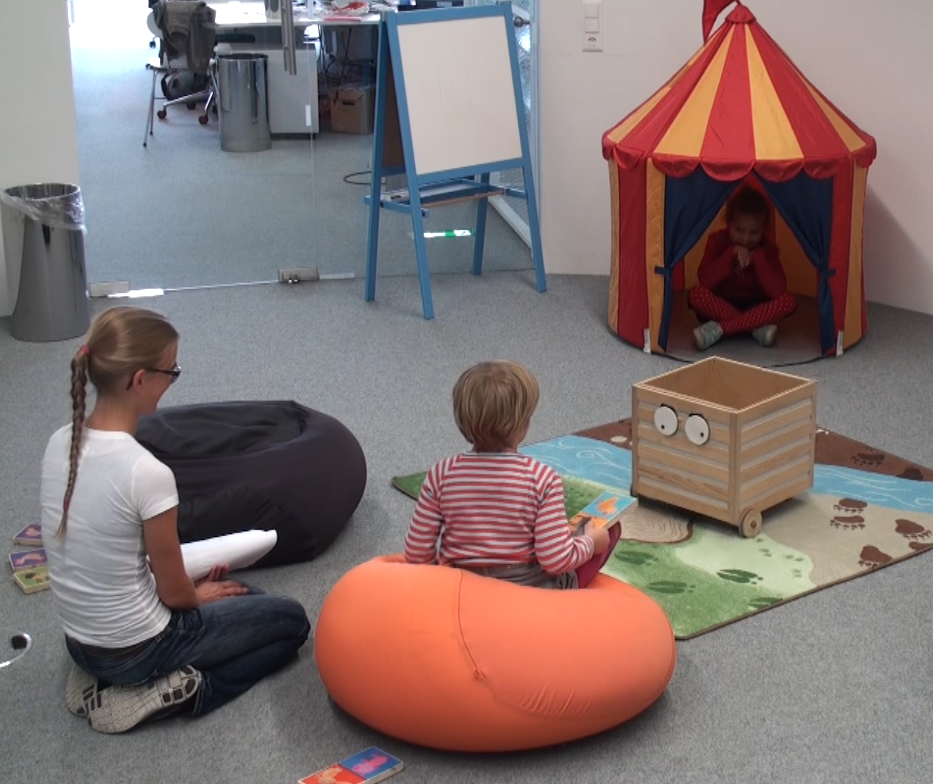
\includegraphics[width=0.5\columnwidth]{domino_header.png} 
    \caption[How do Children Interact with a Robot that Behaves
    Unexpectedly?]{\small \textbf{How do children perceive and interact with a
    robot that behaves unexpectedly?} In an interaction study in the lab, 26
    children aged 4-5 years played with a robot that behaved unexpectedly from time
    to time. We studied children's engagement with the robot and their attributions
    of intentionality to it.}

    \label{fig:domino-header} 
\end{figure}	

\subsection{Research Questions and Hypotheses}

In the Domino Study, we analyze child-robot interaction with a robot that shows
unexpected behavior. In a playful scenario which was set up in a laboratory
environment (Figure~\ref{fig:domino-setup}), 26 children aged 4-5 years were
assembling a domino game together. Each group consisted of two children and the
Ranger robot, which was used to transport domino tiles between the two children.

Ranger usually behaved correctly (expected behavior), coming over to a child
after being called and delivering the domino tile to the other child. However,
in pre-defined rounds Ranger showed unexpected behavior, when a child called the
robot. We defined three different types of \textit{misbehavior} that were tested
in a between-subjects study design:

\begin{itemize}

    \item The robot makes a \textbf{mistake}: When called by the child to come
        over, the robot goes wrong but recognizes its mistake and repairs. We
        expect this to be perceived as \textit{``to err is human''}, and assume
        increased attributions of human-likeness to the robot.\footnote{The
        attribution of human-likeness to a robot is labeled as
        \textit{anthropomorphism}, and we will hereafter sometimes use ``attribute
        intention'' and ``anthropomorphize'' synonymously.} 

    \item The robot gets \textbf{lost}: When called by the child to come over,
        the robot goes wrong, without any observable reason, and remains at the
        wrong location. We expect this to be perceived as a bug or system error
        which causes the robot to not work correctly, and assume few
        attributions of human-likeness to the robot.

    \item The robot \textbf{disobey}: When called by the child to come over, the
        robot shows the intention to not obey by literally ``shaking its head'',
        which should reflect the negative reply to the child's request. The
        robot then goes to a wrong location and remains there while it continues
        to shake its head (this cue is not used in the lost behavior). We expect
        the disobey behavior to be perceived as the robot having an
        \textit{``own will''}, and we assume this leads to increased
        attributions of human-likeness (intention) to the robot.

\end{itemize}	

We analyzed children's reaction focusing on two main aspects. On one hand,
children's \textbf{behavior} (their reactions) toward the unexpected robot
behavior was studied in terms of \textbf{active engagement} with the robot. On
the other hand, we analyzed children's \textbf{perception} of the robot in term
of \textbf{anthropomorphism} -- the attribution of human-like characteristics,
such as cognitive abilities and the ability to show intentions. We assumed that
in general a robot that behaves unexpectedly from time to time can promote
engagement and lead children to attribute intention to it. \cite{short_no_2010}
found that participants anthropomorphize a cheating robot more than a robot that
always behaves fairly, and also evaluate the interaction as more engaging. Based
on the related work we formulate the following two hypotheses:

\begin{description}

    \item[Hypothesis 1:] Children show more engagement toward a robot that
        behaves unexpectedly from time to time compared to a robot that always
        behaves correctly (within subjects variable).

    \item[Hypothesis 2:] Children perceive a robot that shows intention or
        cognitive abilities as more human-like than a robot that appears to have
        a system error, \ie the disobeying robot and the robot that makes a
        mistake will be more anthropomorphized than the robot that gets lost
        (between subjects variable).

\end{description}


Our research questions deal with both children's observable behavior and their
perception of the robot. We would also like to explore the relation between
these two aspects, related to the attribution of human-like characteristics to
the robot. The motivation behind this is to find out whether
\textit{anthropomorphism} cannot only be measured as a specific type of
perception but also as an observable behavior in the interaction itself. Thus,
we would like to take a first step in bringing things together and develop an
\textbf{index of anthropomorphism} that considers both children's perception and
interaction aspects (qualitatively). Previous work suggests that a social
relation to a robot (we view anthropomorphism as a specific type of social
relation) reflects an increased engagement and can be effective in sustaining
interaction. Consequently, we hypothesize a positive correlation between the
anthropomorphic perception of the robot and the amount of engagement in the
interaction.


%\subsection{Engagement}

%\subsection{Unexpected Robot Behavior}

\section{Method and Procedure}

\subsection{Description of the Scenario}

The basic idea of the interaction scenario was that there are two children who
play domino together, with the help of the robotic box Ranger. The scenario
setup is displayed in Figure~\ref{fig:domino-setup}. The challenge is that the
tiles of the domino are distributed in the room, hidden behind three beanbags,
and while one child -- \textit{the searcher} -- searches for the right tile, the
other child -- \textit{the receiver} -- is asked to stay in a play tent. There
is a ``river'' (play carpet) in between the two children that we told them they
cannot cross and therefore they need the robot to transport the domino tiles
between them.

We used a self-made domino consisting of 10 wooden tiles (10~x~20~x~1.5~cm) with
pictures of comic farm animals: cow, sheep, hen, donkey, duck, pig, rabbit. The
pictures were taken from a commercially available domino game adapted to the age
of the children (produced by Djeco, advised age 3+). 

To start the game (divided in several \textit{runs} that correspond each to the
delivery and assembling of one domino tile), there is already one domino tile in
front of the tent, where \textit{the receiver} child stays and assembles the
domino chain. \textit{The receiver} child asks \textit{the searcher} child for a
specific tile, \eg a tile with a donkey, \textit{the searcher} searches for the
respective tile, sits down on the next beanbag, and asks the robot to come over.
The Ranger robot is first located next to the tent, then, when called by the
\textit{searcher} it starts moving, crosses the river carpet, and comes over to
the \textit{searcher} on the beanbag. The \textit{searcher} child puts the
domino tile into the robotic box, and the robot then goes back to \textit{the
receiver} child in the tent. Then, \textit{the receiver} takes out the domino
tile from the robot, and puts the two tiles together. The first \textit{run} is
over, and a new \textit{run} starts, when \textit{the receiver} asks \textit{the
searcher} for the next domino tile.

\subsection{Manipulation of Robot Behavior}
\label{sec:domino-manipulation}

We used the same prototype as in the previous study, and Ranger was again
controlled by a human Wizard, who was in the same room (see
Figure~\ref{fig:domino-setup}). This was to ensure that the Wizard could see
children's interaction and hear their commands to the robot without any delay.
Following a pre-defined script, the robot showed a behavior as presented in the
following list.

\begin{figure}[!b] 
    \centering 
    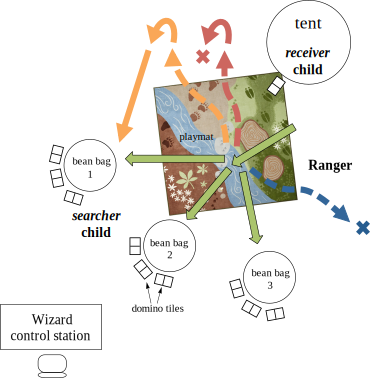
\includegraphics[width=0.9\columnwidth]{domino-setup.pdf} 
    \caption[Study Setup of the Playroom in the Lab]{\small \textbf{Study setup
    of the playroom in the lab (schematic top view)}. We configured one of the
    rooms in the lab to a playroom with a children's tent from IKEA, in which one of
    the children is located (referred to as \textit{the receiver} or ``the child in
    the tent''). A play carpet with a river on it is used as an imaginary barrier
    between the two children. The other child, referred to as \textit{the searcher}
    (or ``the child on the beanbag'') is asked to remain ``on the other side of the
    river'' in the area with the 3 beanbags, behind which each 3 domino tiles are
    distributed (displayed as black stars). In the back of the room, there is a
    camera to record the interaction scenario, and right next to it in the corner,
    there is the Wizard control station: a table with a laptop computer. As some
    parents stayed in the room during the interaction study, they are asked to sit
    on the chairs placed in the back of the room. The board next to the door is not
    used during the experiment, it is simply an accessory. The solid green arrows,
    show the robot's path for the \textit{correct} behavior. The blue dashed arrow
    visualizes a possible \textit{lost} path, where the Ranger stops and remains at
    a wrong stop (denoted by the blue cross). The yellow arrows reflect a possible
    \textit{mistake} path, where the robot goes wrong but then turns toward the
    searcher child (U-turn), and then comes straight over to the searcher. The red
    dashed arrow visualizes a possible \textit{disobey} path where the robot goes
    wrong, then turns toward the child but remains at the wrong stop (red cross).
    The different audio and visual cues that the robot uses during the different
    paths are explained in the text.} 

    \label{fig:domino-setup} 
\end{figure}

The \textbf{correct} robot behavior:

\begin{itemize}

    \item \emph{Domino tile put in robot:} Ranger makes a ``rewarding'' sound
        and shows green light pattern (Figure~\ref{fig:domino-put},
        page~\pageref{fig:domino-put}, the light pattern is still yellow here
        indicating that Ranger ``reached'' the child; the green light pattern
        was shown slightly after the putting was done)

    \item \emph{Domino tile removed from robot:} Ranger makes an ``emptying''
        sound and shows green light pattern (Figure~\ref{fig:domino-remove},
        page~\pageref{fig:domino-remove}).

        %	\item \emph{Box is touched or petted:} Ranger ``blushes'' with pink
        %	light around the area of the box's ``cheeks''

        %	\item \emph{Box is kicked or mistreated:} Ranger makes a
        %	``disturbance'' sound and the box moves backward

    \item \emph{Robot is called by one of the children:} When one of the
        children called the robot saying something like \textit{``Robot come
        here!''}, the robot starts moving toward the child
        (Figure~\ref{fig:domino-call}, page~\pageref{fig:domino-call}). Ranger
        does not react to any other verbal commands.	

    \item \emph{Robot reaches one of the children:} When in front of one of the
        children who should either put or remove a domino tile, Ranger stops and
        shows yellow light, if no reaction, Ranger also makes a wiggle-like move
        (Figure~\ref{fig:domino-show}, page~\pageref{fig:domino-show}).

\end{itemize}

\begin{figure*}[!b]
  \centering

  \subfloat[call]
  {\label{fig:domino-call}
  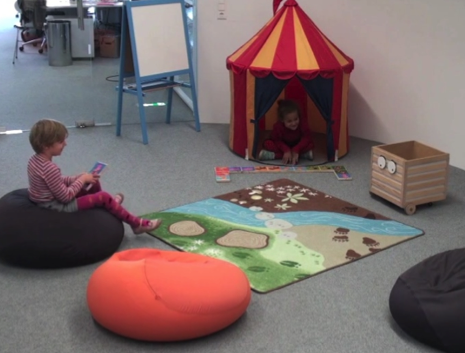
\includegraphics[height=4cm]{domino-call.png}} 
  \subfloat[put]
  {\label{fig:domino-put}
  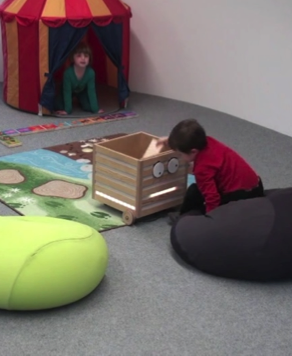
\includegraphics[height=4cm]{domino-put.png}}
  \subfloat[remove]
  {\label{fig:domino-remove}
  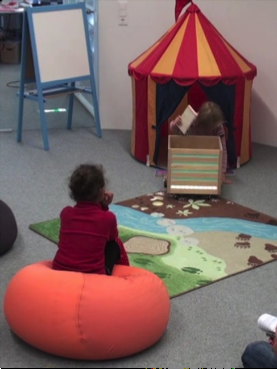
\includegraphics[height=4cm]{domino-remove.png}}  
  
  \bigskip  
  
  \subfloat[explore]
  {\label{fig:domino-explore}
  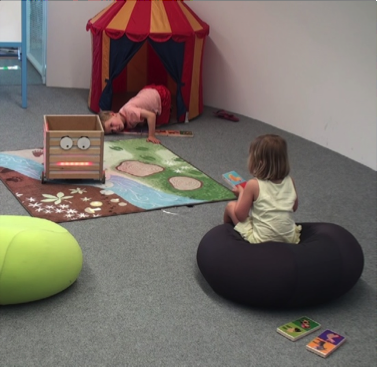
\includegraphics[height=4cm]{domino-explore.png}}
  \subfloat[gesture]
  {\label{fig:domino-gesture}
  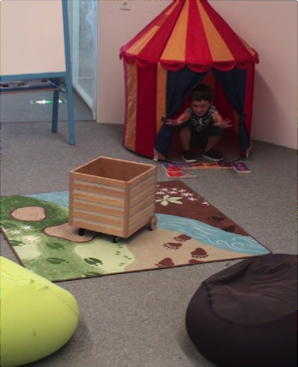
\includegraphics[height=4cm]{domino-gesture.png}}
  \subfloat[misuse]
  {\label{fig:domino-misuse}
  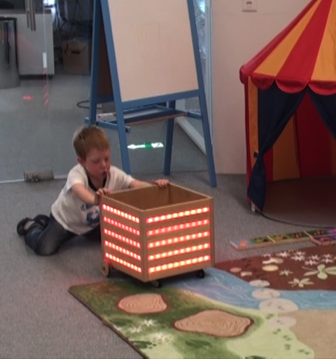
\includegraphics[height=4cm]{domino-misuse.png}}
  
  \bigskip

  \subfloat[show]
  {\label{fig:domino-show}
  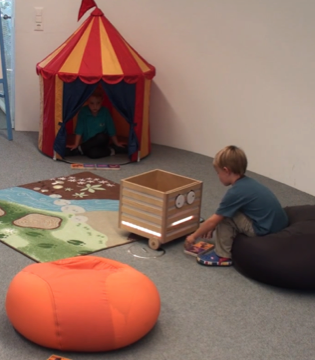
\includegraphics[height=4cm]{domino-show.png}}
  \subfloat[touch]
  {\label{fig:domino-touch}
  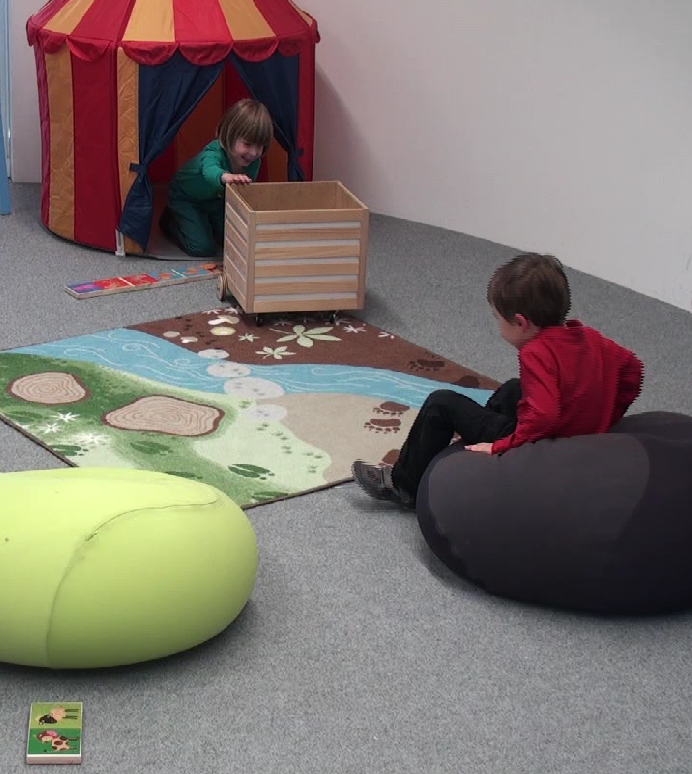
\includegraphics[height=4cm]{domino-touch.png}}   
  \subfloat[look at experimenter]
  {\label{fig:domino-look}
  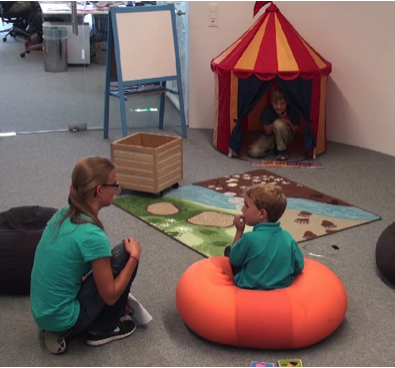
\includegraphics[height=4cm]{domino-look.png}}\\  

  \caption[Children's Interactions with the Robot and the Feedback of the
  Robot]{\small \textbf{Children's interactions with the robot and the feedback
  of the robot.} Apart from \textit{talking} to the robot, which is not
  displayed here, there were nine main interactions, which are explained in the
  respective paragraph on how children's behavior was coded in the videos
  (page~\pageref{sec:domino-coding}). The robot showed feedback to some of the
  children's actions: \textit{call, put} and \textit{remove} (top row), as
  explained in the text.}

  \label{fig:domino-actions}
\end{figure*}	

Most of the time when the sender child (on one of the beanbags, see
Figure~\ref{fig:domino-setup}, page~\pageref{fig:domino-setup}) calls the robot,
it correctly goes right over to the beanbag where the child sits (bold green
arrows in Figure~\ref{fig:domino-setup}). It starts from its starting position
next to the tent, crosses the play carpet with the ``river'' and then goes to
the respective beanbag. During some specific \textit{runs} however, the robot
behaves unexpectedly (dashed arrows in Figure~\ref{fig:domino-setup}). There
were three different \textbf{manipulations} of the robot behavior:

\begin{itemize}	

    \item \textbf{Mistake:} The sender child calls Ranger. The robot goes until
        it is on the carpet, stops, turns, and goes wrong (see yellow path in
        Figure~\ref{fig:domino-setup}). Then, Ranger waits ($\sim$2~sec), turns
        its ``face'' toward the sender child, and ``blushes'' red around its
        ``cheeks'' (as if it recognizes its wrong position,
        Figure~\ref{fig:domino-mistake}, page~\pageref{fig:domino-mistake}).
        Then, Ranger goes correctly over to the sender child. The
        \textit{mistake} behavior is \textit{robot-repaired}, as no
        human-intervention is needed.

    \item \textbf{Lost:} After being called, Ranger goes until it is on the
        carpet. There, it stops, turns, and goes wrong (see blue path in
        Figure~\ref{fig:domino-setup}). Once at the wrong position, Ranger waits
        with its ``face'' turned away from the child, and it blinks in yellow
        light (the same as when in front of a child) (see
        Figure~\ref{fig:domino-lost}, page~\pageref{fig:domino-lost}). Ranger
        remains waiting at the wrong position until the experimenter tells the
        child to go over to the robot to put the domino tile. The \textit{lost}
        behavior is \textit{human-repaired}, as it needs human-intervention.

    \item \textbf{Disobey:} After being called, Ranger goes until it is on the
        carpet. Then, it shows \textit{disobeying} behavior: It stops, makes red
        light all over its surface and produces a repeated ``disturbance''
        sound. It turns, and goes to a wrong position (see red path in
        Figure~\ref{fig:domino-setup}). Still blinking in red, it turns its
        ``face'' toward the sender child (Figure~\ref{fig:domino-disobey},
        page~\pageref{fig:domino-disobey}). In addition to the red blinking,
        Ranger makes a slow wiggle-like move, and remains waiting at the wrong
        position until the experimenter tells the child to go over to the robot
        to put the domino tile. Also the \textit{disobey} behavior is
        \textit{human-repaired}.	

\end{itemize}	


\begin{figure}[!t]
  \centering
\subfloat[mistake]
  {\label{fig:domino-mistake}
  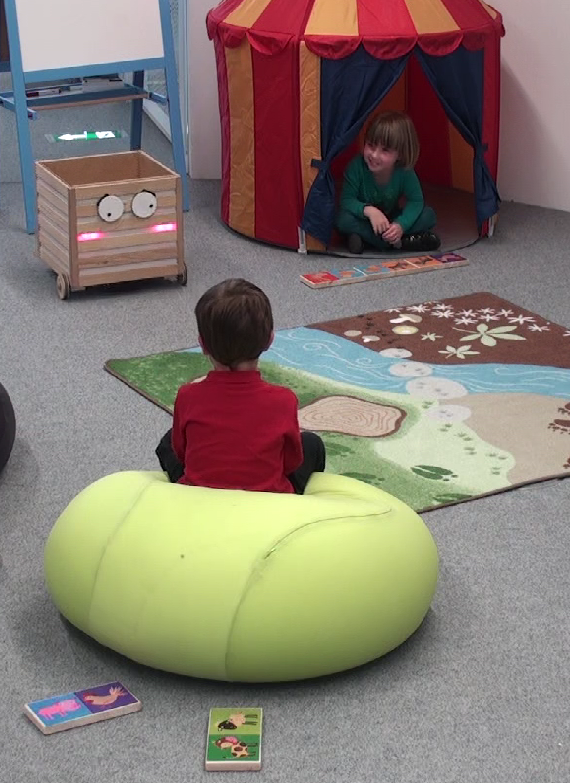
\includegraphics[height=5cm]{domino-mistake.png}}
  \subfloat[lost]
  {\label{fig:domino-lost}
  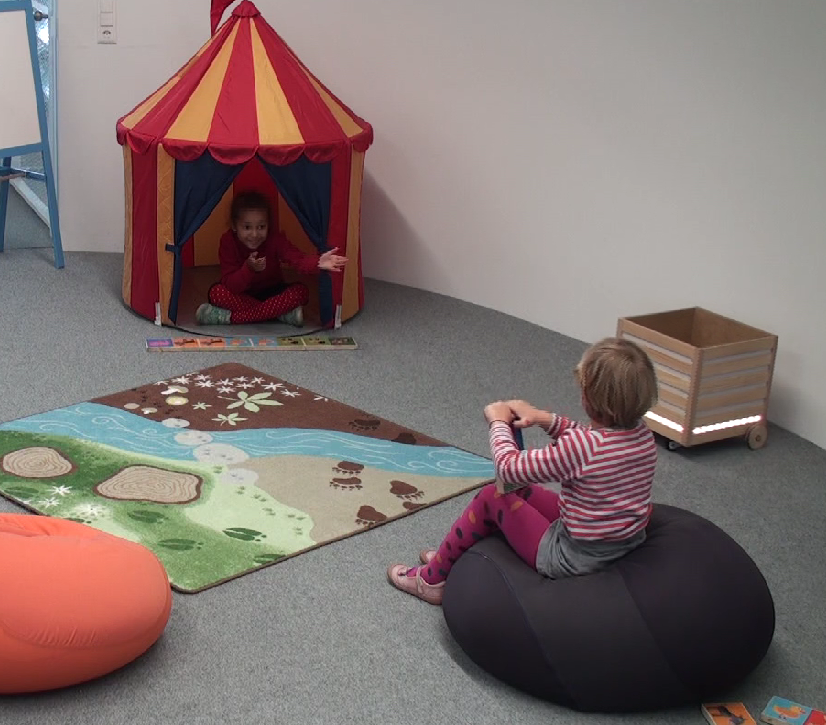
\includegraphics[height=5cm]{domino-lost.png}}
  \subfloat[disobey]
  {\label{fig:domino-disobey}
  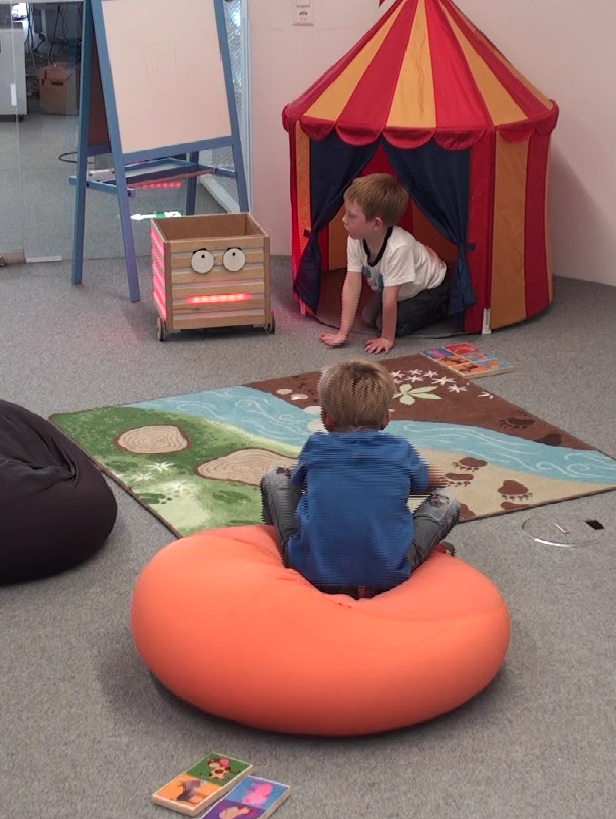
\includegraphics[height=5cm]{domino-disobey.png}}

  \caption[The Three Robot Misbehaviors]{\small \textbf{The three robot
  misbehaviors.}}

  \label{fig:domino-misbehavior}
\end{figure}

On its way back to the tent, Ranger always goes correctly. After the sender
child has put a domino tile, Ranger automatically turns and goes over to the
tent (the receiver child does not even need to call the robot).

%\paragraph{Time points of robot misbehavior}

After several correct runs, we assumed that children expect consistent robot
behavior. When the robot then does something unexpected, children are likely to
be positively surprised. A similar effect has been observed in a study with a
robot that was cheating from time to time \cite{short_no_2010}.

It may be that children interpret the unexpected robot behavior as a failure.
But we do not want them to lose trust in the robot, contrary, the unexpected
robot behavior should have a positive effect and promote engagement. We tried to
avoid a negative influence by timing the robot misbehavior not at the very
beginning and very end of the interaction, because it has been shown that early
and late robot failures negatively impact trust
\cite{desai_effects_2012,desai_impact_2013}. Desai et al. suggest that users
should all start and end with a working system. Consequently, we placed several
unexpected robot behaviors around the middle of the interaction, as shown in
Table~\ref{tab:domino-second}.

Also \cite{short_no_2010} decided to follow this pattern when introducing
unexpected robot behavior. In their study with a robot that cheated, from the 20
rounds of the rock-paper-scissors game, the robot cheated three times in the
middle: on the 4th, 8th and 15th round. The authors adjusted the interaction
length so that the spacing and timing of the cheating was preserved.

In our study, there were 14 runs in total. 5 runs were used to set the baseline
and in those 5 runs the robot always behaved correctly. Then, in the 9 remaining
runs, the robot showed misbehavior at the $3^{rd}$ and $4^{th}$ run as well as
at the $7^{th}$ and $8^{th}$ run (see Tables~\ref{tab:domino-first} and
\ref{tab:domino-second} on page \pageref{tab:domino-first}).	

\subsubsection{Scenario Description}

\subsubsection{Manipulation of Robot Behavior}

\subsubsection{Semi-structured Interviews with Children}

\subsubsection{Participants}

Overall, there were 13 pairs of children (n=26) participating in the interaction
study: 16 boys and 10 girls, 4-5 years old (M=4.46, SD=0.45). In 11 of the
pairs, children were friends who knew each other from kindergarten, nursery
school or because they lived in the same neighborhood. 2 of the pairs were
composed of brother and sister.

Table~\ref{tab:domino-sample} (page~\pageref{tab:domino-sample}) gives an
overview.

\begin{table}[H]
%\vspace{1 cm}
\captionof{table}[Domino Study Participants]{\small \textbf{Overview of the 13 groups (n = 26 children) that participated in the Domino Study.} The \textit{scenario duration} is the time that children spent interacting with the robot. The time duration of the short interviews is not included here. The \textit{anthropomorphism index} is a score that we developed and which measures how far children anthropomorphize the robot during the interaction study and the interview (see Section~\ref{sec:domino-anth-score}). The last row of the table gives the overview of the sample including the Mean age (M), the average scenario duration and average anthropomorphism index.}
\label{tab:domino-sample}       % Give a unique label
\centering
\footnotesize

\begin{tabular}{lllll}
\hline\noalign{\smallskip}
	\multirow{3}{*}{\textbf{group}} & \multirow{3}{*}{\textbf{children (age)}} & \multirow{3}{*}{\textbf{relation}} & \textbf{scenario} & \textbf{anthropomorphism} \\
	 & & & \textbf{duration} & \textbf{index} \\
	 & & & (min:sec) & points / \% \\
\noalign{\smallskip}\hline\hline\noalign{\smallskip}

	mistake1 & boy (4) & friends & 19:01 & 5.75 / 36~\% \\ 
	& boy (4) & & & \\ 
\noalign{\smallskip} \hline \noalign{\smallskip}

	mistake2 & boy (5) & friends & 15:28 & 10 / 63~\% \\
	& boy (4.5) & & & \\ 
\noalign{\smallskip} \hline \noalign{\smallskip}

	mistake3 & boy (4) & family & 15:24 & 8 / 50~\% \\ 
	& girl (4) & & & \\ 
\noalign{\smallskip} \hline \noalign{\smallskip}

	mistake4 & boy (4.5) & friends & 13:23 & 8 / 50~\% \\ 
	& girl (4.5) & & & \\ \noalign{\smallskip} \hline \hline \noalign{\smallskip}

	lost1 & boy (4.5) & family & 17:08 & 8.75 / 55~\% \\ 
	& girl (4.5) & & & \\ \noalign{\smallskip} \hline \noalign{\smallskip}

	lost2 & boy (5) & friends & 16:43 & 8.75 / 55~\% \\
	& boy (4.5) & & & \\  
\noalign{\smallskip} \hline \noalign{\smallskip}

	lost3 & girl (4.5) & friends & 15:01 & 7.5 / 47~\% \\ 
	& girl (4.5) & & &  \\ \noalign{\smallskip} \hline \noalign{\smallskip}

	lost4 & boy (5) & friends & 13:04 & 8.25 / 52~\% \\
	& girl (4) & & & \\ 
\noalign{\smallskip} \hline \hline \noalign{\smallskip}

	disobey1 & boy (4.5) & friends & 13:37 & 3.75 / 23~\% \\
	& girl (4.5) & & & \\ \noalign{\smallskip} \hline \noalign{\smallskip}

	disobey2 & boy (4.5) & friends & 17:37 & 3.25 / 20~\% \\ 
	& girl (4.5) & & & \\ \noalign{\smallskip} \hline \noalign{\smallskip}

	disobey3 & boy (5.5) & friends & 17:38 & 10.25 / 64~\% \\ 
	& boy (5.5) & & & \\ \noalign{\smallskip} \hline \noalign{\smallskip}

	disobey4 & girl (4) & friends & 14:46 & 4.5 / 28~\% \\
	& girl (4) & & & \\ \noalign{\smallskip} \hline \noalign{\smallskip}

	disobey5 & boy (4) & friends & 16:25 & 10.75 / 67~\%  \\
	& boy (4) & & & \\
\noalign{\smallskip} \hline \hline \noalign{\smallskip}
	
	13 groups & M age 4.46 & 2 family & 15:47 & M 7.5 / 47~\% \\ 
	26 children & 16 boys, 10 girls & 11 friends & & (SD 2.5 points) \\	
\noalign{\smallskip}\hline

\end{tabular}
\end{table}	

\subsubsection{Course of the Study}

We recruited pairs of children (4-5 years old, who knew each other) to play a
``collaborative domino game with a robot''. We distributed flyers in the campus
kindergarten, sent out mails to pre-schools in town, and made a posting on an
online-blog that targets parents in Lausanne.

Participants were invited to come to our lab for a playful child-robot
interaction study that would last 60 min at most. Parents (or guardians) brought
their children and could either stay in the arranged play room or go to the
cafeteria in the same building. During the study, two experimenters were
present.

\begin{itemize}

    \item \textbf{Introduction and pre-interview ($\sim$5~min):} One of the
        experimenters introduced the study to the parents and asked them to sign
        a consent form. The other experimenter briefed children by explaining
        them the domino game and conducting the pre-interview (questions about
        previous experience with robots, and their expectations)\footnote{The
        interview questions for all three short-interviews are given in
        Table~\ref{tab:domino-questions} and the original French version can be
        found in the Appendix (page~\pageref{apx:domino-interview}).}. At the end of the
        pre-interview we introduced the Ranger box (first hidden under the wizard table)
        and explained that it was there to transport the domino tiles between them.

    \item \textbf{First interaction phase ($\sim$10~min):} In all 5 runs the
        robot behaves correctly, as displayed in Table \ref{tab:domino-first}.
        This first interaction phase was the same across all three conditions.
        It serves to familiarize children with the situation, the robot, and the
        game. We can assume that children expect consistent robot behavior
        afterwards.

\begin{table}[H]
\captionof{table}[First Interaction Phase (5 Runs with Correct Robot Behavior)]{\small \textbf{First interaction phase.} The robot behaved correctly~(v) in all five runs.}
\label{tab:domino-first}       % Give a unique label
\centering
\footnotesize
\begin{tabular}{lccccc}
\noalign{\smallskip}\noalign{\smallskip}\hline\noalign{\smallskip}
	&  run 1.1 & run 1.2 & run 1.3 & run 1.4 & run 1.5  \\ 
\noalign{\smallskip}\hline\hline
	\textit{correct} & v & v & v & v & v  \\ 
\noalign{\smallskip}\hline
\end{tabular}
\end{table}

    \item \textbf{First short interview ($\sim$5~min):} In this interview we
        asked children several questions to assess their first impression of
        Ranger, and how far they ascribe cognitive abilities and mental states
        to the correctly behaving robot. After this first interview, children
        switched their roles (beanbag / tent), so to create a balance.

    \item \textbf{Second interaction phase ($\sim$20~min):} In the 9 runs of the
        second phase, the robot alternated between behaving correctly and
        misbehaving, as displayed in Table \ref{tab:domino-second}.
	
\begin{table}[H]
\captionof{table}[Second Interaction Phase (9 Runs with Partly Robot Misbehavior)]{\small \textbf{Second interaction phase.} There are 9 runs in the second interaction phase. At some time points, namely runs 2.3, 2.4 and 2.7, 2.8., the robot showed the respective misbehavior~(x), according to the experimental group either \textit{mistake, lost} or \textit{disobey}. In the other runs, namely runs 2.1, 2.2. and 2.5, 2.6 and 2.9 the robot behaved correctly~(v).}
\label{tab:domino-second}       % Give a unique label
\centering
\footnotesize
\begin{tabular}{lccccccccc}
\noalign{\smallskip}\noalign{\smallskip}\hline\noalign{\smallskip}
	&  run 2.1 & run 2.2 & \textbf{run 2.3} & \textbf{run 2.4} & run 2.5 & run 2.6 & \textbf{run 2.7} & \textbf{run 2.8} & run 2.9 \\ 
\noalign{\smallskip}\hline\hline
	\textit{mistake} & v & v & \textbf{x} & \textbf{x} & v & v & \textbf{x} & \textbf{x} & v \\ 
	\textit{lost} & v & v & \textbf{x} & \textbf{x} & v & v & \textbf{x} & \textbf{x} & v \\ 
	\textit{disobey} & v & v & \textbf{x} & \textbf{x} & v & v & \textbf{x} & \textbf{x} & v \\
\noalign{\smallskip}\hline
\end{tabular}
\end{table}

    \item \textbf{Second short interview ($\sim$5~min):} After this phase of
        interacting with the unexpectedly behaving robot, we conducted another
        short interview and a debriefing with the children. We mostly asked
        open-ended questions, concerning several topics, such as whether they
        noticed anything unusual in the robot behavior (manipulation check), and
        how far they ascribe cognitive abilities, mental states, and moral
        standing to the robot after it had shown unexpected behavior.  

\end{itemize}

In the end, we thanked parents and children and each child received a little
gift (\eg a small puzzle or a coloring book). Some children made a drawing of
the robot, which may be an interesting qualitative evaluation tool for future
studies with young children.

%	when there was enough time (we set a time limit of 60 min as duration for the entire experiment), we asked children to draw the Ranger robot with which they had just played. 	

The study was set up as a between-subjects experiment with three conditions,
corresponding to the three types of robot misbehavior. Thus, in one group the
robot only showed one type of misbehavior during the second interaction phase.
There were each 4 groups in the \textit{mistake} and \textit{lost} condition,
and 5 groups in the \textit{disobey} condition (see
Table~\ref{tab:domino-sample}). We did not have a control condition in which the
robot always behaved correctly in all 14 runs. However, we consider the first 7
runs as reference for \textit{expected behavior} (runs 1.1-2.2), to compare
against the remaining 7 runs, reflecting \textit{unexpected behavior} (2.3-2.9,
manipulation phase with the 3 conditions). As such, we can carry out a
within-subjects analysis to investigate the difference between expected and
unexpected robot behavior. All interactions and interviews were video and
audio-recorded.

\subsection{Semi-structured Interviews with the Children}	

It is not easy to interview young children. We have seen this in our previous
study. Children have a short attention span, we (the experimenters) are
strangers to them, and they are in an unfamiliar environment. The pre-interview
served to ``break the ice'' and during the first playful interaction phase, most
children familiarized themselves with the situation.

Also, children do not articulate themselves and understand questions like
adults. We tested our interview structure and the script in a pilot-study with
three young children, and were assisted in formulating our questions by a
pedagogue and father of four. This helped us adapting our language and
question-style to the 4-5 year old participants. We set up the interviews like a
casual conversation / discussion, so we did not separate the two children in
order to keep the situation natural. We used casual and informal language
adapted to the age of the children, and encouraged them to justify their answers
and tell us more details by asking, for example, \textit{How do you know ... ?}
or \textit{Tell me, what have you observed when ... ?}. We paid attention to not
``put words in children's mouth''. Consequently, though we re-phrased and
repeated some questions, we never forced children to give an answer, and
accepted when they said they would not know or when they did not respond at all.	

\begin{table}[h]
%\vspace{1 cm}
\captionof{table}[Questions Used During the Interviews with Children]{\small \textbf{Questions used during the semi-structured interviews with children.} An ``X'' indicates if the question was used in the pre-interview (\textit{pre}), in the \textit{first} short interview (after the 5 runs in which the robot behaved correctly) or in the \textit{second} short interview (after the 9 runs in which the robot sometimes showed unexpected behavior). The Ranger robot toy box is abbreviated with ``R''. (The original French version of the interview script is in the Appendix, page~\pageref{apx:domino-interview}.)}
\label{tab:domino-questions}       % Give a unique label
\centering
\footnotesize
\begin{tabular}{lcccl}
\hline\noalign{\smallskip}
	\textbf{question} & \textbf{pre} & \textbf{first} & \textbf{second} & \textbf{construct} \\
\noalign{\smallskip}\hline\hline\noalign{\smallskip}

	How do you imagine a robot? & X & & & \multirow{3}{*}{expectation} \\
	What could it look like? & X & & & \\
	Have you ever seen a robot before? & X & & & \\
\noalign{\smallskip} \hline \noalign{\smallskip}

	When you first saw R, what did you think? &  & X & & \multirow{4}{*}{impression} \\
	Is R a robot? How do you know? & & X & & \\
	Did you expect R would come over to you when you call it? & & X & & \\
	What happened when you put the domino tile in the box? & & X & & \\
\noalign{\smallskip} \hline \noalign{\smallskip}

	Do you think R could go out the door all by itself? & & X & & \multirow{4}{*}{ascribe intention} \\	
	Does R always obey / come over to you? & & X & X & \\
	Could R do something silly? & & X & X & \\
	Why did R not come over to you when you called it? & & & X & \\
\noalign{\smallskip} \hline \noalign{\smallskip}

	Here is a domino tile. Do you think R can see it? & & X & X & \multirow{2}{*}{ascribe cognitive abilities} \\
	When I say \textit{``Hello R!''}, do you think R can hear it? & & X & X & \\	
\noalign{\smallskip} \hline \noalign{\smallskip}

	Does R have feelings? Can R be happy or sad sometimes? & & & X & ascribe emotional state \\
\noalign{\smallskip} \hline \noalign{\smallskip}	
	
	Do you like R? Why (not)? & & & X & \multirow{3}{*}{social acceptance} \\
	What do you (not) like about it? & & & X & \\
	Would you like to have R at home? & & & X & \\	
\noalign{\smallskip} \hline \noalign{\smallskip}	
	
	Could R be your friend? Why (not)? & & & X & companionship\\
\noalign{\smallskip} \hline \noalign{\smallskip}		
	
	Assume you go on a holiday for two weeks. Is it alright & & & \multirow{2}{*}{X} & \multirow{2}{*}{ascribe moral standing}\\
	~~to leave R alone at home? Why (not)? & & &  & \\	
\noalign{\smallskip}\hline

\end{tabular}
\end{table}		

We generally needed to keep the interviews as short as possible. In designing
our interview script and selecting relevant questions, we took inspiration from
previous work on child-robot interaction and children's perception of robots
\cite{kahn_jr._robotic_2006,weiss_i_2009,leite_influence_2013}. For instance, we
applied and adapted some of the ``constructs'' and example questions from the
questionnaires used in \cite{kahn_jr._robotic_2006} and \cite{weiss_i_2009}. The
authors evaluated children's perception of the robotic dog AIBO after the
children had played with the robot. A ``construct'' addresses a specific factor
(topic) that can be measured by several questions. For instance, the construct
``cognitive abilities'' (called ``cognition'' in \cite{weiss_i_2009}) considers
the robot's ability to hear and to see (perceptual skills), as attributed by the
children. The construct ``moral standing'' and the respective question was taken
from \cite{kahn_jr._robotic_2006}.\footnote{According to
\cite{kahn_jr._robotic_2006}, \textit{moral} refers to considerations based on
an artifact's physical or psychological welfare, and virtue (whether the
artifact deserves care). An attribution of moral standing reflects, for
instance, that the robot engenders moral regard, is morally responsible,
blameworthy, has rights or deserves respect.}			Similarly, we grouped
questions according to specific constructs that they evaluate (see
Table~\ref{tab:domino-questions}). This was an adaption and extension of the
questions and constructs used in previous work.\\

With several recurring questions in the first and second interview, we wanted to
see the differences in children's perception of the correctly behaving and
unexpectedly behaving robot. We planned to use these two interviews as a
within-subject measurement, however, this did not work out very well because
children's responses were not always accurate, not comparable one by one, and
children did not always give an answer.	


%	Even when children reply that they do not know, this is interesting. Then we either do not ask a good question or they are really uncertain about it.


Similar to how we processed interviews in the previous studies, we qualitatively
transcribed interviews, \ie we did not craft a full word-by-word transcript but
noted down any statement that was useful and relevant. This was organized in a
spreadsheet, so to obtain an overview of the different replies to a question.
The interviews were analyzed in a qualitative manner.	


\subsubsection{Measurements, Coding and Data Analysis}

We have obtained two main types of data. On one hand, as just described, we can
analyze children's verbal statements concerning their \textbf{perception of the
robot} (captured in the audio recorded interviews). On the other hand, what we
describe in the following paragraphs, we can do a quantitative and qualitative
analysis of \textbf{children's behavior toward the robot} (captured in the video
recordings). Furthermore, we can investigate how far these two types of data can
be used to understand children's engagement in the interaction and how far they
anthropomorphize the robot. We would like to develop a toolkit that considers
both children's perception and interaction, in order to measure anthropomorphism
(as a special type of human-like engagement with the robot).	

\paragraph{Coding children's behavior in the videos}	
\label{sec:domino-coding}	

Similar to the coding scheme we used in the Ranger study
(Chapter~\ref{chap:Ranger-fieldstudy}), we annotated children's behavior in the
videos. Snapshots of the actions, along with the robot's feedback are shown in
Figure~\ref{fig:domino-actions}, page~\pageref{fig:domino-actions}. For the
segmentation of behavior we also used the same method as in the Ranger study. We
coded 10 different actions:	
	
\begin{itemize}

    \item \textbf{Explore (ex)}: when children actively try to find out what the
        robot is doing (\eg by looking under the box); attentively watch or
        observe the robot (\eg attentively waiting for the box to show a
        reaction); experiment with the robot to figure out how it works (\eg put
        hands in front or inside of the box to see what happens);

    \item \textbf{Misuse (mis)}: when children kick the robot, poke it in its
        ``eye'', try to climb on or inside the box, drive / push the robot
        around, stop the robot's wheels with a foot;\\

    \item \textbf{Put domino (put)}: when a domino tile is put inside the box;

    \item \textbf{Remove domino (rem)}: when a domino tile is removed from the
        box;

    \item \textbf{Gesture (ges)}: when gestures are used to communicate /
        interact with the robot (\eg pointing gestures, waving at the robot);

    \item \textbf{Touch (touch)}: when the box is touched (\eg petted or
        caressed);

    \item \textbf{Show (show)}: when a child shows something to the robot (\eg
        by holding a domino tile in front of its eyes);

    \item \textbf{Call (call)}: when a child calls the robot to come over;

    \item \textbf{Talk (talk)}: when a child directly talks to the robot (using
        direct speech) besides calling the robot;

    \item \textbf{Look (look)}:	when a child looks at the experimenter due to
        confusion caused by the robot; look is not coded when the experimenter
        asks a question to the child;

\end{itemize}	

The actions \textit{put, remove} and \textit{call} were ``requested'' actions
because the scenario required them and children were asked to carry them out.
Hence, these actions are not relevant to be analyzed quantitatively. The other
actions \textit{explore, misuse, gesture, touch, show, talk} and \textit{look}
are spontaneous actions that were not requested but arose in the interaction.
Hence, these actions are interesting to study, and they can further be used to
analyze \textbf{engagement}.


\subsubsection{Analyzing engagement with Ranger}

%	\textbf{Engagement} is a key metric in social HRI. In general, there are two
%	types of engagement: emotional and behavioral engagement.  efficacy of
%	various social characteristics (emotion, dialogue, personality \etc) can be
%	measured for capturing attention (acquisition time) and holding interest
%	(duration) \citep{steinfeld_common_2006}.	
	
%	In a long-term interaction study with 8-9 year old children,
%	\cite{leite_long-term_2013} was measuring engagement through video
%	observations (by analyzing the amount of time that children spent looking at
%	the robot), interviews, and questionnaires. The interviews were
%	semi-structured, containing initial yes-or-no questions followed by
%	open-ended questions that allowed children to justify and elaborate their
%	answers.
%We have chosen a similar approach: in video observations we coded the action
%\textit{explore}, which includes carefully watching the robot. We also
%conducted short-term interviews with the 4-5 year old children, however,
%questionnaires were not feasible with this age group.

There are different possibilities to measure engagement in HRI, depending on the
specific research question and context. Metrics to measure behavioral engagement
in the interaction include, for instance, conversation analysis (\eg used in
\cite{short_no_2010}) or general attention analysis. These can be studied by
analyzing interaction videos in terms of head movement, eye tracking and gesture
/ body movement analysis (\eg in \cite{sidner_explorations_2005}).
Post-measurements to measure emotional engagement can be questionnaires that try
to assess constructs like the perceived presence and involvement in the
interaction. An example is the \textit{Interactive Experience Questionnaire}
(originally developed by \cite{lombard_measuring_2000}) of which adapted
versions were used in
\cite{kidd_effect_2004,bainbridge_effect_2008,short_no_2010}.

A mix of several methods has been used in a long-term interaction study with 8-9
year old children, \cite{leite_long-term_2013}. The author measured engagement
through video observations (by analyzing the amount of time that children spent
looking at the robot), interviews, and questionnaires. The interviews were
semi-structured, containing initial yes-or-no questions followed by open-ended
questions that allowed children to justify and elaborate their answers. We have
chosen a similar approach that considers both children's behavioral and
emotional engagement.	

%	: in video observations we coded several ``engagement actions
%	\textit{explore}, which includes carefully watching the robot. We also
%	conducted short-term interviews with the 4-5 year old children, however,
%	questionnaires were not feasible with this age group.

With 4-5 year old children, however, we cannot use rating scales to ask them
about constructs as abstract as social presence or how much they felt involved
in the interaction. Here, we rely mostly on video analysis to quantify
engagement. Several of the aforementioned coded actions
(Section~\ref{sec:domino-coding}) can reflect engagement: \textit{explore,
misuse, gesture, touch, show,} and \textit{talk}. Also, \textit{look} at the
experimenter can be considered as engagement in the interaction: We assume that
children look at the experimenter when they are surprised and seek for help.
This behavior reflects that they want to make sense of the robot's behavior and
that they notice it as ``strange''. Further, we can take into account how they
refer to Ranger and describe the robot (as well as their experience) in the
interviews. We describe the combination of the two types of data in the next
paragraphs.


\paragraph{Engagement reflected in the perception of the robot}

We assume that active reasoning about Ranger reflects engagement (or interest in
the robot). But how do we identify whether children, 4-5 years old, reason about
a robot, its cognitive abilities, intentions or mental states, rather than
viewing it as a machine stepping through a task? As \cite{short_no_2010}
mentioned: \textit{``It is not easy to measure the attribution of mental
state.''} Asking \textit{``How much does the robot think?''} is not sufficient.
Short et al. proposed to rely more on subtle cues in the participants' behavior
and responses. The nature of participants' responses to open-ended question
about the robot's behavior (whether they noticed anything unusual and what) can
give insight into their attributions of mental state to the robot.

%	In \cite{short_no_2010}, a speech analysis revealed that participants used
%	more active voice verbs to describe the behavior of the cheating robot
%	compared to the robot that behaved fairly at all times. The authors
%	interpret that a use of active voice implies action in choice, and
%	attributions of mental state to the robot.

In terms of children's perception of Ranger, we used some of the questions
presented in Table~\ref{tab:domino-questions} to assess how far they
anthropomorphize the robot. As an indication for anthropomorphism we take
questions in the constructs \textit{ascribe intention, ascribe cognitive
abilities, ascribe emotional state}, and \textit{ascribe moral standing}.


\paragraph{Engagement reflected in the interaction}	

As previously mentioned, from the 10 types of actions that were coded in the
videos, we cannot consider all of them as reflecting engagement with Ranger.
Since we asked children from our side to \textit{call} the robot, as well as to
\textit{put} and \textit{remove} domino tiles, these three actions were
excluded. Finally, we consider the following 7 actions as \textbf{engagement
actions}: \textit{explore, misuse, gesture, touch, show, talk}.\footnote{In
several figures of the ``engagement actions'' later on, \textit{explore} is
excluded from the visualization because it was too prominent and differences in
the other actions would not be observable. The huge proportion of
\textit{explore} suggests that this category needs to be refined in future
studies.}



\paragraph{Anthropomorphism index}
\label{sec:domino-anth-score}

To account for the fact that anthropomorphism arises in an interaction, we try
to bring both children's perception of the robot (post-measurement) and their
behavior toward it (in-the-moment measurement) together. By doing so, we would
like to obtain a qualitative \textbf{anthropomorphism index}. We quantify the
index by giving 1 point for each anthropomorphic perception of the robot (max.
13 points) and for specific kinds of human-like behavior toward the robot (max.
3 points). The index included the following aspects:\\ \\

\textbf{Perception: \textit{(max. 13 points)}}
\begin{itemize}
	\item Ascribe \textbf{mental states / feelings} to Ranger: \textit{0-4 points}\\
	(2 points for agreeing that Ranger can be happy or sad; 2 points for attributing Ranger with hunger or tiredness)
	\item Ascribe \textbf{cognitive abilities / intention} to Ranger: \textit{0-4 points}\\ 
	(each 0.5 points for ascribing seeing and hearing ability; 1 point for agreeing that Ranger can go out the door by itself; 1 point for disagreeing that Ranger always obeys; 1 point for agreeing that Ranger can do something silly)
	\item Ascribe \textbf{sociality / companionship} to Ranger: \textit{1 point}\\ 
	(1 point for agreeing that Ranger can be a friend)
	\item Ascribe \textbf{moral standing} to Ranger: \textit{1 point}\\ (1 point for disagreeing that Ranger be left alone at home)
	\item Other \textbf{anthropomorphic statements}: \textit{0-3 points}\\ 
	(1 point for anthropomorphic reason for Ranger's misbehavior; 2 points for anthropomorphic reason for not leaving Ranger alone) 
\end{itemize}

\textbf{Behavior: \textit{(max. 3 points)}}
\begin{itemize}
	\item Use of \textbf{direct speech} toward Ranger: \textit{1 point}\\
	(\textit{calling} the robot to come over is not considered)
	\item Use of \textbf{polite formulations} toward Ranger: \textit{1 point}\\ 
	(\eg saying \textit{``thank you Ranger''} or \textit{``please Ranger ...''} or \textit{``goodbye''})
	\item Use of \textbf{social or pointing gestures} toward Ranger: \textit{1 point}\\ 
	(\eg waving at the robot, nodding)
\end{itemize}
	
There are certainly limitations to this scoring scheme. For instance, the
balance between perception and behavior aspects is questionable (13 to 3
points). Also, we did not consistently assign 1 point to each item, but assigned
points between 0.5 and 2 points. We did this because we found that different
items reflect a higher level of anthropomorphic perception of the robot than
others (for instance, ascribing the ability to see an hear was suggested by our
study setup, and we cannot be sure that it really reflects anthropomorphism).
There are possibilities of refinement of this scoring scheme. For instance, a
more systematic weighting procedure and the identification of all relevant
factors would be an interesting future achievement. We could introduce a formula
to calculate the anthropomorphism index \textit{$\alpha$} by taking the sum of
the various items ($x_1, x_2, x_3...$) and different weights ($a, b, c ...$) to
balance them: $\alpha$ \textit{=} $a x_1$ \textit{+} $b x_2$ \textit{+} $c x_3
...$~. Machine learning techniques could be used to optimize such a calculation
of the anthropomorphism index.


\section{Findings}

There are two main types of findings: 1) related to the interaction of the
children with the robot and 2) related to the perception of the robot. This
section is organized accordingly. We then bring both types of data together by
building the \textit{anthropomorphism index}. 

\subsection{Interaction}

\paragraph{Scenario and run duration}

In total, there was more than 5~hours of video material obtained from the
13~groups. The video material consisted of around 3.5~hours of the two
interaction phases and 1.5~hours of interviews. The interaction analysis
considers only the video parts that correspond to the \textit{scenario
duration}, which starts when the receiver child in the tent asks the searcher
child for the first domino tile, and it stops when the receiver child puts
together the last domino to the chain. The scenario duration is split in two
interaction phases, as described in Section \ref{sec:domino-course-study}, with
a pause in the middle, that corresponds to the first interview. On average, the
first interaction phase with 5 runs of the always correctly behaving robot
lasted 5~min~34~sec. The second interaction phase with 9 runs and the partly
misbehaving robot lasted on average 10~min~14~sec. Overall, the scenario
duration (all 14 runs) varied between 13~min~04~sec and 19~min~01~sec (average
15~min~47~sec, SD~=~1~min~50~sec). The condition had no significant impact on
the scenario duration (F(2,23)=.18, p=.835).\\

When looking at the average duration of each run, it is not a surprise that the
runs in which the robot misbehaved (2.3-2.4 and 2.7-2.8) lasted longer
(M~=~71~sec, SD~=~16~sec) than the runs in which the robot behaved correctly
(M~=~54~sec, SD~=~16~sec). Overall, for the runs with the correctly behaving
robot, there is a tendency that the average duration of the run decreases over
time ($M_{run1.1}$~=~73~sec, $M_{run2.9}$~=~42~sec). This suggests that children
familiarize themselves with the playful task and the robot and react more
promptly to it.


\paragraph{Interaction}
	 
\begin{figure}[!h]
  \centering
\subfloat[total number (count, \%)]    
    {\label{fig:domino-action-count}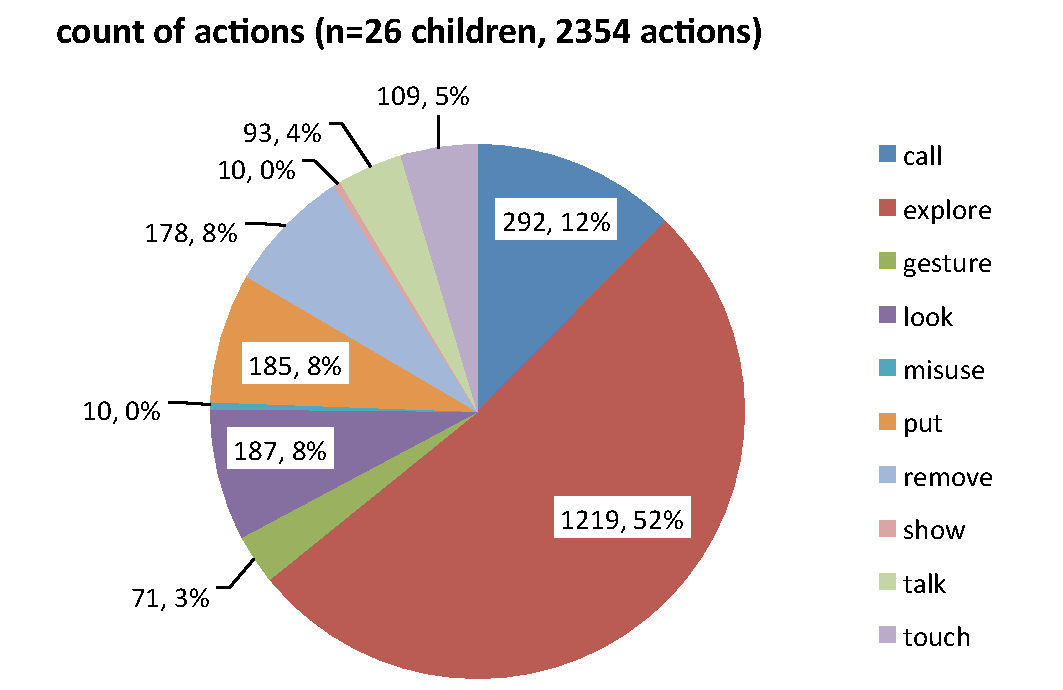
\includegraphics[height=5cm]{domino_actions-pie.pdf}}
%  \hspace{0.3cm}
\subfloat[annotation duration, (\%)]    
    {\label{fig:domino-action-time}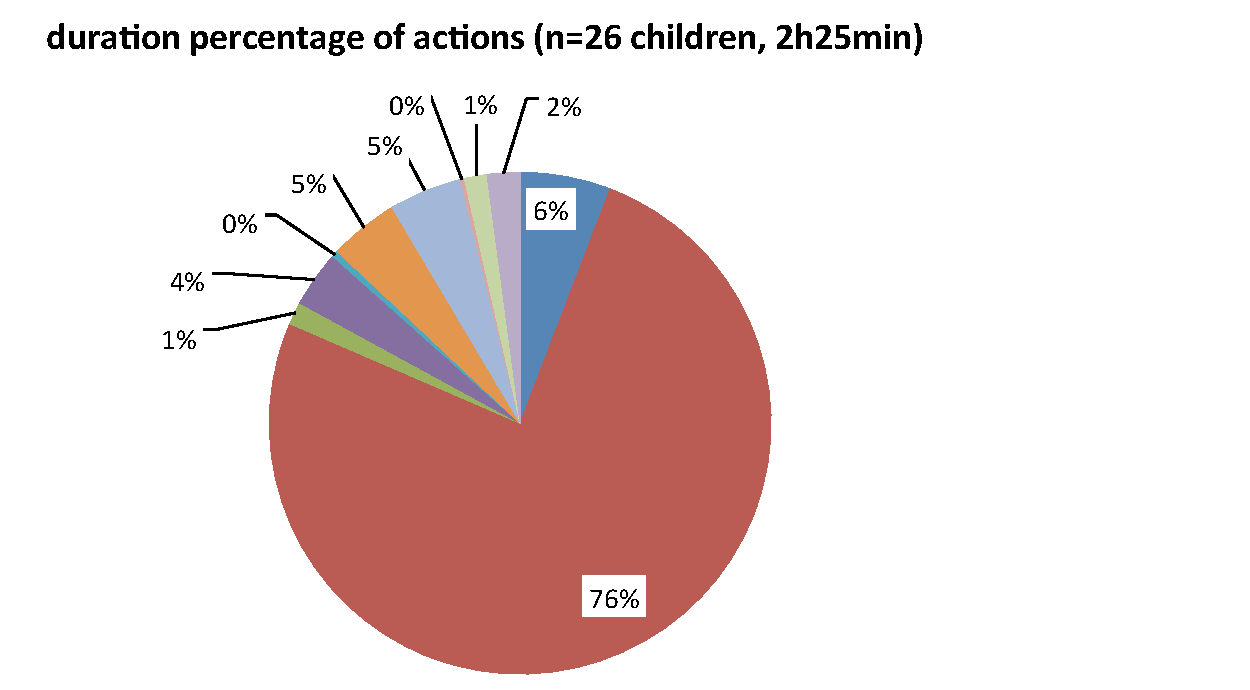
\includegraphics[height=5cm]{domino_duration-pie.pdf}}

  \caption[Total Number and Duration of Children's Actions with Ranger]{\small \textbf{Children's actions with Ranger.} (a) shows the total number of the counted actions that were annotated in the videos, (b) shows the total annotation duration percentage of these actions (the total duration of all coded actions are considered as 100\%, not the duration of the scenario).}
  \label{fig:domino-actions-pie}
\end{figure}		 

After having coded children's actions in the video, we obtained 2354 distinct
actions which summed up to a total annotation duration of 145 minutes. On
average, one child accounted for 92 actions (SD=23). The average number of
actions carried out per child was less in the \textit{disobey} condition
(average 75 actions) than in the \textit{lost} (average 98 actions) and
\textit{mistake} (average 102 actions) condition. The overall distribution of
the count of actions and the duration of the total annotation time per action is
shown in Figure~\ref{fig:domino-actions-pie}. We see that even more than in the
previous study, \textbf{children explored the robot} (52~\% of the actions,
making up 76~\% of the total annotation duration). Exploring includes carefully
watching the robot or actively trying to find out how it works. For instance,
one boy (4 years, group \texttt{lost1}) clapped his hands and waved in front of
Ranger's eyes; then he told the experimenter \textit{``No, it cannot hear and it
doesn't see me!''}.\\ 

Overall, the interactions with the robot were less varied than in the previous
study. We assume this was because the scenario was not as open but fairly well
structured and probably even more constrained (compared to the previous study
which was carried out in children's own rooms).

%	Also, children were asked to remain in the tent and around the beanbag, so
%	they could not freely interact with Ranger, as it was possible in the field
%	study. This constraint is alright because the Domino Study does not openly
%	explore interactions but focuses on children's reaction to the misbehaving
%	robot. 

Besides \textit{explore}, children engage mostly in the actions required by the
scenario (Figure~\ref{fig:domino-actions-pie}): \textit{call} (12~\%),
\textit{put} (8~\%) and \textit{remove} (8~\%). Another 8~\% of the actions were
\textit{look} at the experimenter, which suggests that children were seeking for
help or reinforcement sometime. The remaining 12~\% of actions are attributed to
\textit{touch} (5~\%), \textit{talk} (4~\%) and \textit{gesture} (3~\%). 


\begin{figure}[!b] 
\centering 
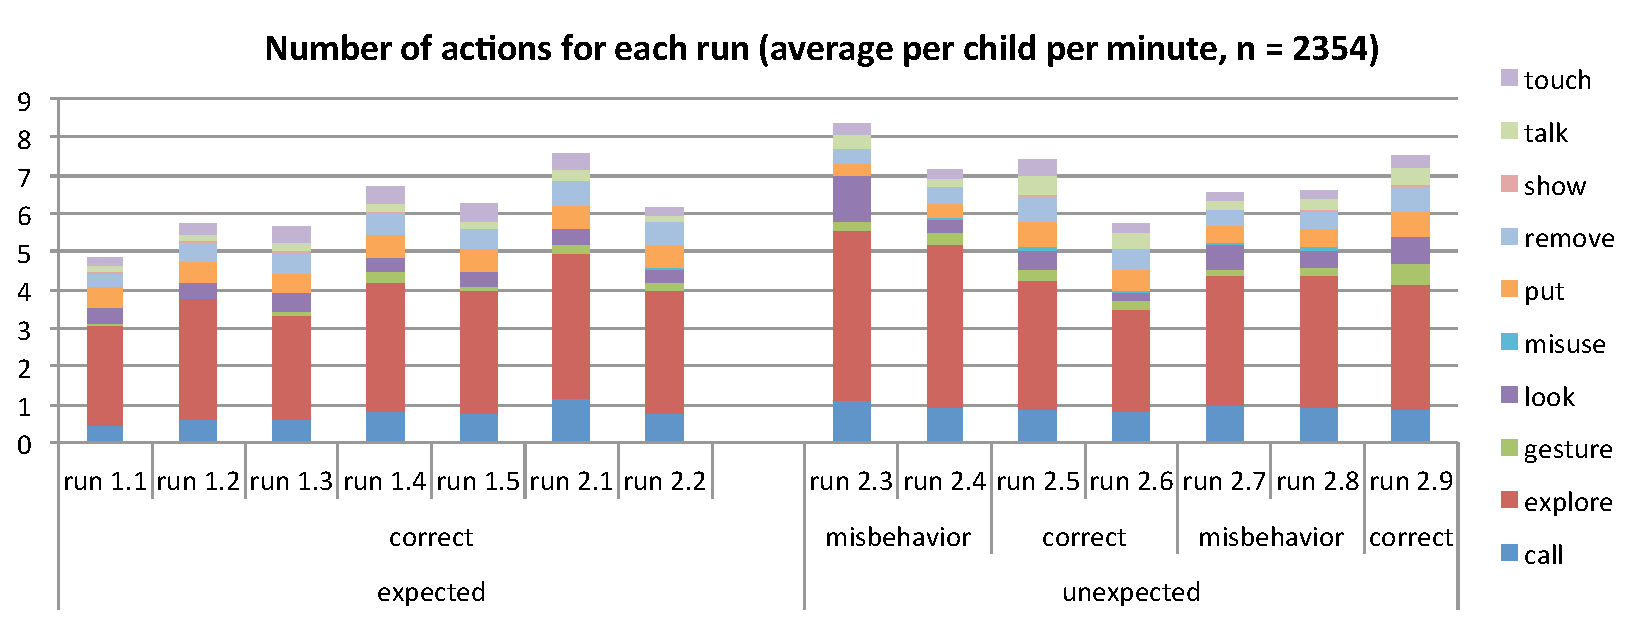
\includegraphics[width=0.99\columnwidth]{domino-time-all.pdf} 
\caption[Number and Type of Actions for Each Run]{\small \textbf{Number and type of actions for each run} (average for one child per minute). Generally, the number of actions does not decrease over time (from run 1.1 to run 2.9). The first 7 runs correspond to the \textit{expected phase}, the second 7 runs correspond to the \textit{unexpected phase}. Especially during run 2.3, the first time when the robot showed an unexpected behavior, children tended to \textit{look} more at the experimenter. During the unexpected phase, also \textit{talk} and \textit{gesture} seem to be increased. The specific values comparing the expected and unexpected phases overall are presented in Table \ref{tab:domino-conditions}, page~\pageref{tab:domino-conditions}.}
\label{fig:domino-time-all} 
\end{figure}		

When visualizing the average count of \textbf{actions for each run} (see
Figure~\ref{fig:domino-time-all}), we can see that over time, the total number
of actions does \textit{not} decrease. While interacting with the expected
behaving robot, there is a peak in run 2.1 which may be due to the fact that
children switched roles before that run. During the interaction with the
unexpected behaving robot, there are peaks in runs 2.3, the first run in which
the robot misbehaved, and a small peak in run 2.9, the very last run. This last
peak may be due to the fact that we told children this was the last run, and as
most children did not want to stop playing with the robot. Hence, they tended to
show some extra engagement, by increasing their use of \textit{gestures} and
\textit{talking} to the robot, for instance.

The key question is: how was the interaction impacted by the three
\textbf{different robot misbehaviors}?
Figure~\ref{fig:domino-time-condition-one} shows how the number of actions
evolved from run to run by condition. Overall, children tended to interact
slightly less with the \textit{disobeying} robot (the actions are normalized,
\ie they show an average per child per minute). This difference can be observed
during all the runs (and has also been found concerning children's engagement
with the robot, see next paragraphs). We are not sure how to interpret this. We
have to assume that interaction differences between the groups and further
individual differences between the children are the reason. We come back to
individual differences in the interaction later.  


\begin{figure}[!h] 
\centering 
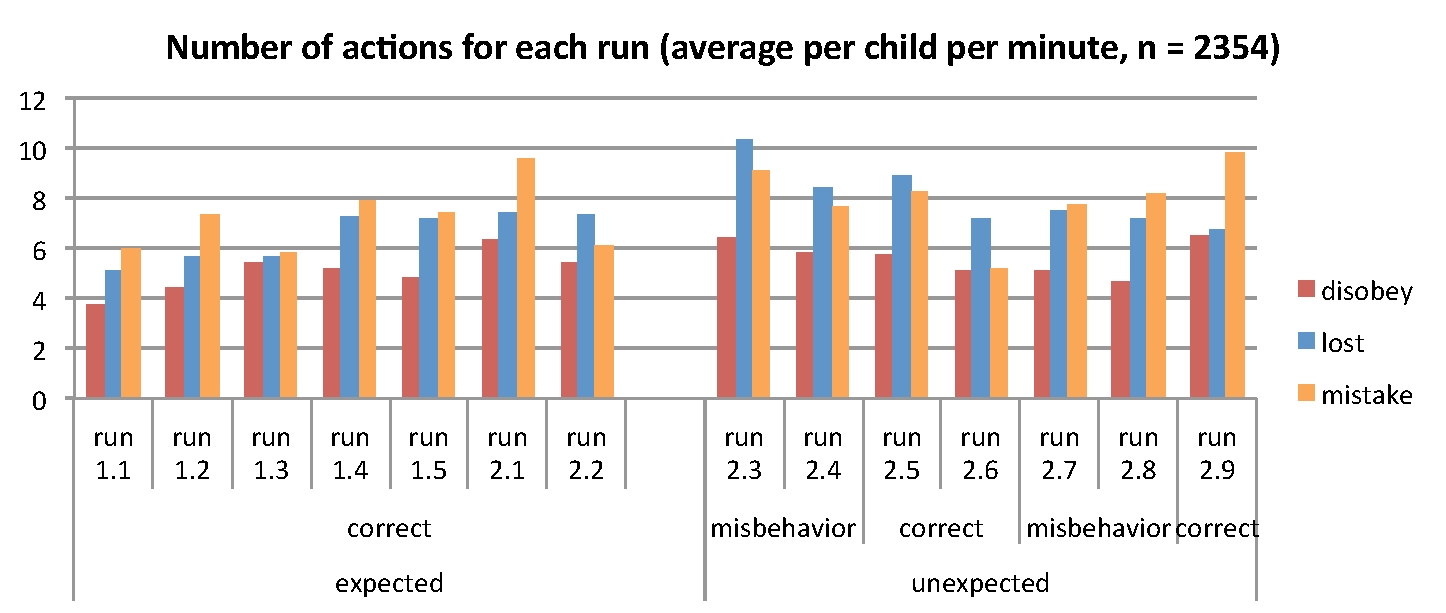
\includegraphics[width=0.9\columnwidth]{domino-actions-perrun.pdf} 
\caption[Total Number of Actions for Each Run per Condition]{\small \textbf{Total number of actions for each run per condition} (average for one child per minute). Generally, the number of actions does not decrease over time (from run 1.1 to run 2.9). Especially during run 2.3, the first time when the robot showed an unexpected behavior, children interact more with the robot, as well as during run 2.7 when the robot misbehaved again after two correct runs. Another increase of actions is during the very last run.}
\label{fig:domino-time-condition-one} 
\end{figure}		
 

When comparing children's interaction with the robot between the
\textit{expected} phase and the \textit{unexpected} phase, the differences
between the conditions and the effect of the robot's misbehavior in general,
become clearer. Table~\ref{tab:domino-conditions} gives an overview. It compares
the number of actions in the expected and unexpected phase for the different
robot behaviors (average per child). The only two actions that were
significantly impacted by the different robot manipulations were
\textit{explore} and \textit{look}. As these two actions are considered to
reflect engagement, we will come back to these differences in the next
paragraphs on engagement with the robot. Overall, the values indicate that
children interacted on average more with the robot in the \textit{lost} and
\textit{mistake} condition. Also, in most cases, the values are higher in the
unexpected phase than in the expected phase. Consequently, children interacted
more during the phase with the misbehaving robot than during the phase when the
robot always behaved correctly. (Statistical tests to compare the effect of the
three different robot behaviors are provided in the following paragraphs,
concerning the \textit{``engagement actions''}, which are subset of all the
interactions.)


\begin{table*}[H]
\captionof{table}[Actions with the Three Robot Misbehaviors in Expected and Unexpected Phase.]{\small \textbf{Comparison of actions with the three robot misbehaviors in the expected and unexpected phase}. This table is based on n~=~2354 counted actions, and shows the average scores per child for the different actions by robot behavior condition. The first line in each double-row shows the values for the expected (exp) phase, in the second line are the values for the unexpected (unexp) phase. For instance, a value of 5.13 for \textit{call} in the expected phase, means that a child called the robot on average 5 times during the expected phase. Italic numbers indicate higher value when comparing the values of the expected and unexpected phase within the condition. Bold numbers indicate highest values when comparing the three different conditions.}
\label{tab:domino-conditions}       % Give a unique label
\centering
\footnotesize
\begin{tabular}{lcccccccccc}
\noalign{\smallskip}\noalign{\smallskip}\hline\noalign{\smallskip}
	 & \textbf{call} & \textbf{explore} & \textbf{gesture} & \textbf{look} & \textbf{misuse} & \textbf{put} & \textbf{remove} & \textbf{show} & \textbf{talk} & \textbf{touch} \\ 
	 & exp & exp & exp & exp & exp & exp & exp & exp & exp & exp \\
	 & unexp & unexp & unexp & unexp & unexp & unexp & unexp & unexp & unexp & unexp \\
\noalign{\smallskip}\hline\hline
	
	\textit{mistake} & \textbf{5.13} & \textbf{26.25} & 0.63 & 3.63 & 0.00 & \textit{\textbf{3.88}} & 3.00 & 0.00 & 0.50 & \textit{\textbf{3.00}} \\
	(n=813) & \textit{6.50} & \textit{\textbf{31.75}} & \textit{\textbf{2.50}} & \textit{4.38} & \textit{0.25} & \textbf{3.50} & \textit{\textbf{3.63}} & \textit{\textbf{0.38}} & \textit{2.25} & \textbf{2.63} \vspace{0.2cm} \\ 

	\textit{lost} & 3.63 & 25.00 & 0.63 & \textbf{3.88} & 0.00 & 3.50 & \textbf{3.50} & \textit{\textbf{0.50}} & 0.38 & 0.75 \\
	 (n=787) & \textit{\textbf{6.88}} & \textit{31.38} & \textit{1.75} & \textit{\textbf{6.88}} & 0.00 & \textbf{3.50} & 3.50 & 0.00 & \textit{1.75} & \textit{1.00} \vspace{0.2cm} \\
	
	\textit{disobey} & 5.00 & 12.00 & \textbf{1.30} & 1.20 & \textbf{0.10} & \textit{3.70} & \textit{\textbf{3.50}} & 0.10 & \textbf{2.50} & \textit{2.90} \\
	(n=754) & \textit{6.70} & \textit{19.50} & \textit{1.40} & \textit{2.70} & \textit{\textbf{0.80}} & 3.40 & 3.40 & \textit{0.20} & \textit{\textbf{3.00}} & 2.00 \\

\noalign{\smallskip}\hline
\end{tabular}
\end{table*}	


\paragraph{Engagement with the robot}	
\label{sec:domino-engagement}

In terms of \textbf{engagement}, the novelty of the robot certainly plays a role
here. As mentioned before, the findings here do not directly address the issues
of long-term usage but concern short-term \textit{engagement}, which is a
pre-requisite for long-term usage.


The huge proportion of \textit{explore} actions (52~\% of all coded actions)
already suggests that children were generally engaged in the interaction, and
most of the time carefully observed what the robot did. When considering the
actions \textit{explore, gesture, look, misuse, show, talk}, and \textit{touch}
as \textbf{engagement actions}, 1699 of the 2354 actions reflected engagement
(72~\%). This indicates that overall children were very engaged in the
interaction with the robot. Furthermore, data suggests that the robot in the
\textit{mistake} and \textit{lost} condition were more engaging for children
(each 75~\% of the actions reflected engagement) than the robot in the
\textit{disobey} condition (66~\% reflected engagement). The statistical
analysis supports this: An ANOVA indicates that there was a significant effect
of robot behavior on the actions \textit{explore} (F(2,23)=11.31, p<.001) and
\textit{look} (F(2,23)=4.6, p=.021). Post-hoc comparisons using the Tukey's test
indicate that the mean score for \textit{explore} in the \textit{disobey}
condition is significantly different from the score in the \textit{mistake} and
\textit{lost} condition. This suggests that children explored the disobeying
robot less\footnote{It is surprising that the disobeying robot was explored
less. One may assume that the disobeying robot might better attract children's
attention because it faces the searcher child and uses fairly strong audio and
light cues as compared to the other behaviors.} (for the average values, see
Table~\ref{tab:domino-conditions}). For \textit{look}, the only significant
difference is found between the mean scores of \textit{lost} and
\textit{disobey}. Data suggests that when the robot is lost, children look more
often at the experimenter than when the robot disobeys. The other actions were
not found to differ significantly between the robot behavior conditions.	

Overall, was there an effect on engagement when the robot misbehaved? We compare
children's engagement during the interaction phase with the expected robot
behavior and during the interaction phase with the unexpectedly behaving robot.
A statistical analysis revealed a significant difference between the average of
engagement actions carried out during the first 7 runs (correct robot behavior)
and during the second 7 runs, when the robot behaved unexpectedly (F(1,36)=5.1,
p=.03). Figure~\ref{fig:domino-engagement-condition} shows the values for
engagement actions in the three conditions, comparing the expected and
unexpected phase. In all three conditions, children carried out more engagement
actions with the unexpectedly behaving robot. No interaction effect was found
between the two phases of interaction (expected / unexpected) and condition
(F(2,36)=1.2, p=.31). In general, this finding supports our first hypothesis:
children show more engagement toward a robot that behaves unexpectedly from time
to time compared to a robot that always behaves correctly.

It is, however, unclear why children engaged less with the disobeying robot (as
mentioned before), especially also in the \textit{expected} phase (see
Figure~\ref{fig:domino-engagement-condition}). In this phase, the robot did not
disobey but always behaved correctly as in the other two conditions. There were
no robot behavior differences between the conditions. We have to assume that the
effect is due to individual and group variations of children's behavior. These
individual variations would probably be less observable in the data if the
sample size would have been bigger.

\begin{figure}[!t] 
\centering 
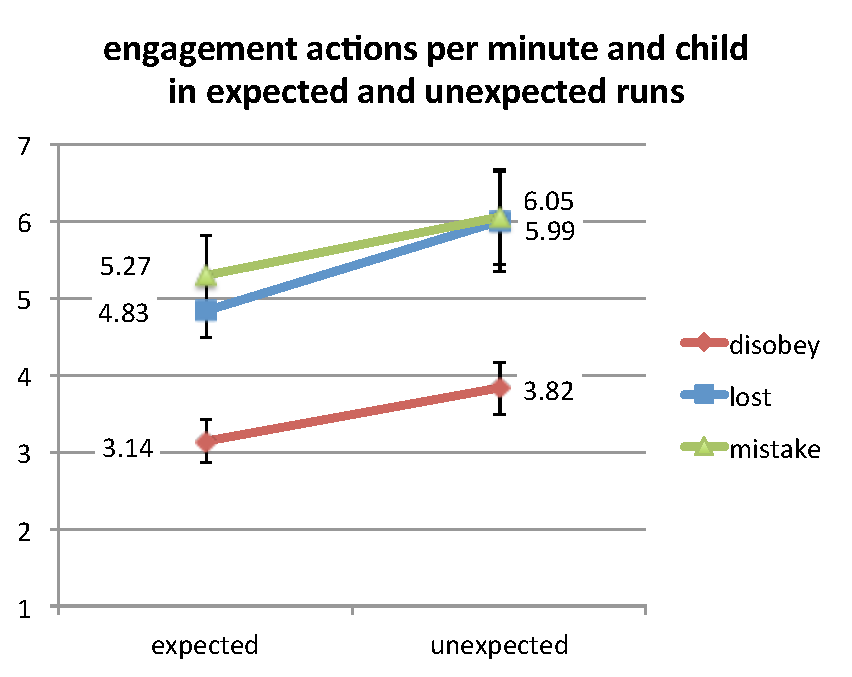
\includegraphics[width=0.5\columnwidth]{domino-engagement-condition.pdf} 
\caption[Engagement Actions in Expected and Unexpected Phase]{\small \textbf{Average number of engagement actions in expected and unexpected phase.} In all three behavior conditions, children engage more in the unexpected phase. In general, the \textit{lost} and \textit{mistake} misbehavior are more engaging than the \textit{disobeying} behavior.} 
\label{fig:domino-engagement-condition} 
\end{figure}	
	
Looking into detail, how did engagement change from run to run?
Figure~\ref{fig:domino-time-active} shows the average engagement actions
(without explore) for each run. How can we explain these variations? During the
\textit{first interaction phase} with the \textit{expected behavior}, we observe
small variations. Then, with the first \textit{unexpected robot behavior} in run
2.3, there is a huge peak in the engagement actions, which can again be observed
in run 2.5, slightly in run 2.7, and then again in the last run 2.9. These runs
correspond exactly to when the robot changed its behavior form correct to
incorrect and \textit{vice versa}. It appears that children are quite sensitive
to these variations and spontaneously respond to it. But as mentioned before, we
have to note that the huge peak of engagement actions in the last run may be due
to the fact that children knew this was going to be the last round.

\begin{figure}[!h] 
\centering 
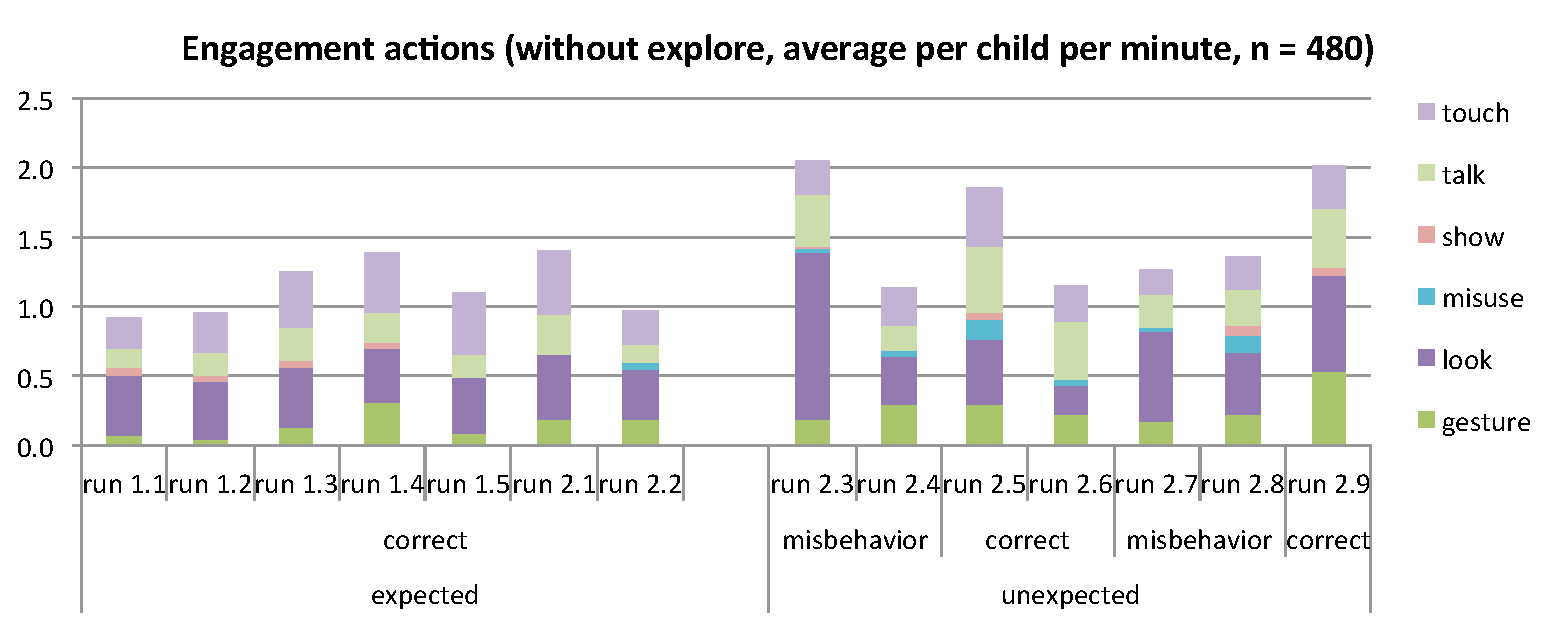
\includegraphics[width=0.99\columnwidth]{domino-time-active.pdf} 
\caption[Engagement Actions for Each Run]{\small \textbf{Engagement actions for each run} (without explore). Average for one child per minute.}
\label{fig:domino-time-active} 
\end{figure}

The picture is unclear, when looking at how engagement evolved from run to run
in the three different conditions (see Appendix
Figure~\ref{fig:domino-time-condition},
page~\pageref{fig:domino-time-condition}). Both within the respective conditions
and when comparing them, there are variations that are difficult to make sense
of and we cannot give a clear interpretation how these variances may be related
to the respective robot misbehavior. We have to assume that the fairly small
sample size of 8-10 children per condition and the huge differences in
children's individual interaction style is the reason for these strange
variations.

Overall, our data suggest that the robot that gets lost and does a mistake
engage in a similar way but that the disobeying robot elicits less engagement.
This was verified by computing an average value for the \textit{engagement
actions}. This average expresses how many engagement actions one child did per
minute. The general engagement action values of the \textit{mistake} (5.66) and
\textit{lost} (5.41) condition are higher than the value of the \textit{disobey}
(3.48) condition. This shows again, that the disobeying robot was less engaging
for the children. A possible interpretation of this result is, that the
disobeying robot frustrated children or was perceived more negatively than the
other two manipulations.

\begin{figure}[!h]
    \centering
    \subfloat[disobey3, boy S15]    
    {\label{fig:domino-diff-group1}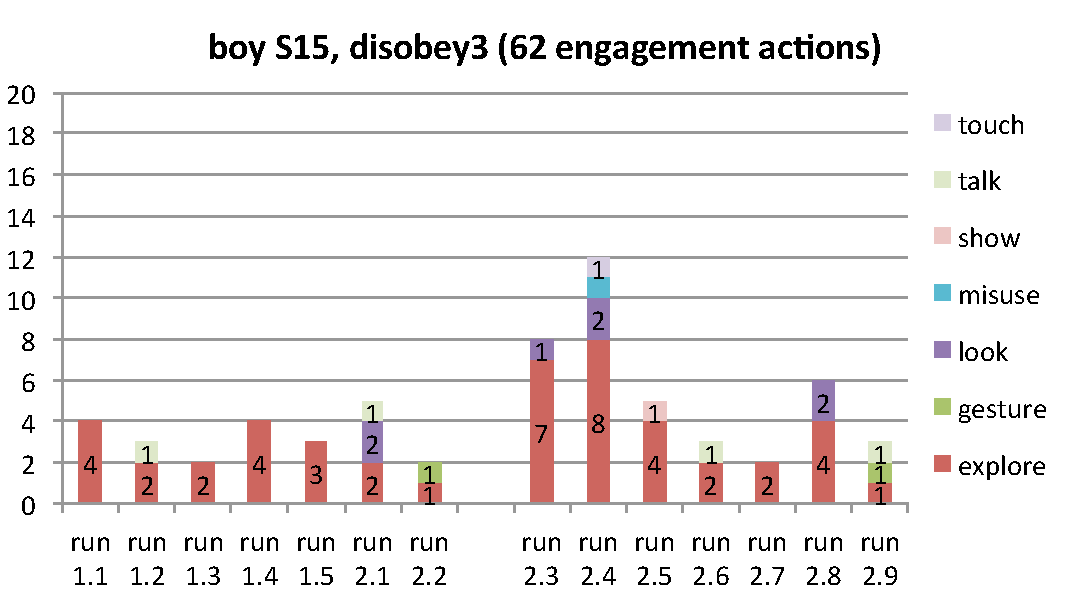
\includegraphics[height=4cm]{domino-disobey3_S15.pdf}}
    %  \hspace{0.3cm}
    \subfloat[disobey3, boy S16]    
    {\label{fig:domino-diff-group2}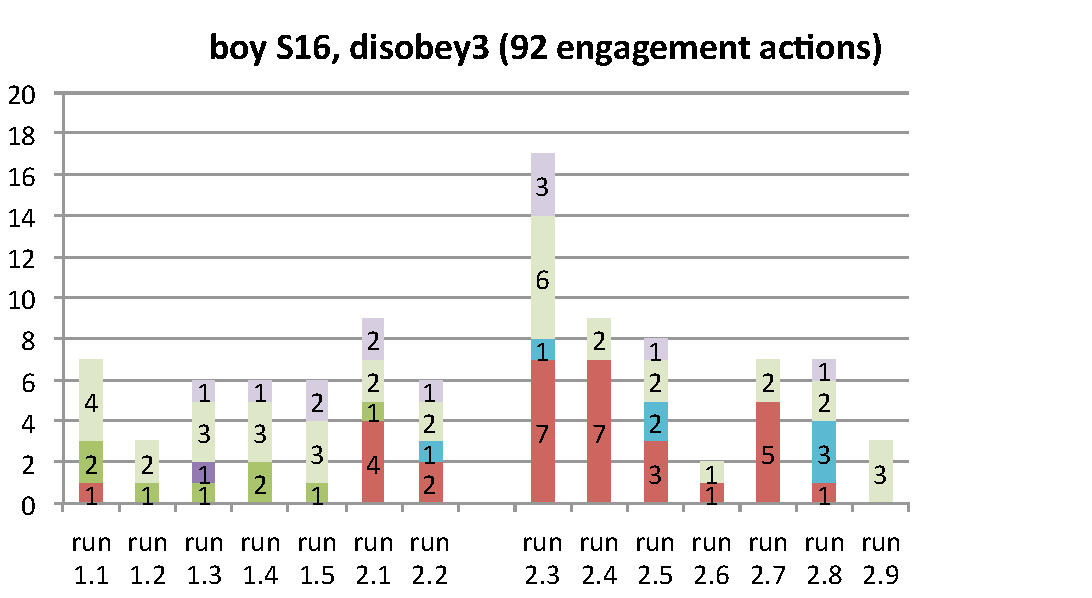
\includegraphics[height=4cm]{domino-disobey3_S16.pdf}}\\
    %  \hspace{0.3cm}
    \subfloat[mistake1, boy S5]    
    {\label{fig:domino-same-group1}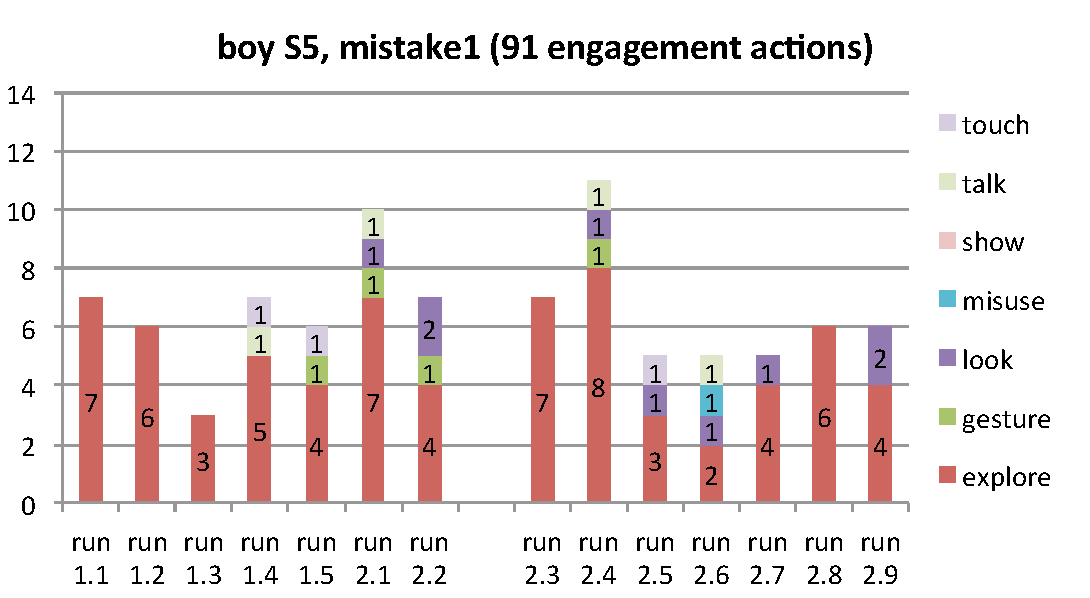
\includegraphics[height=4cm]{domino-mistake1_S5.pdf}}
    %  \hspace{0.3cm}
    \subfloat[mistake1, boy S6]    
    {\label{fig:domino-same-group2}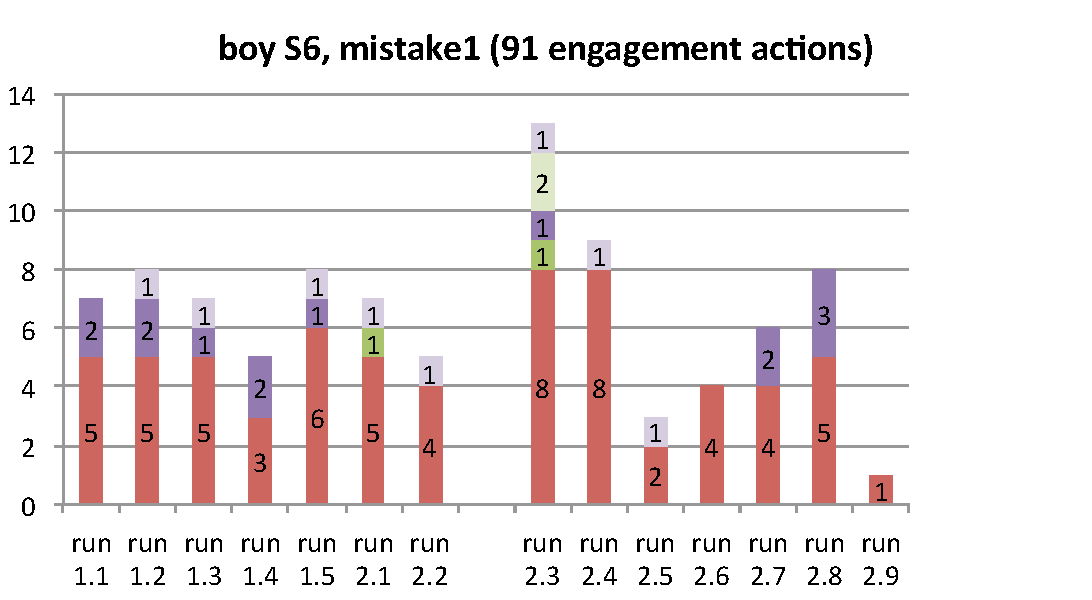
\includegraphics[height=4cm]{domino-mistake1_S6.pdf}}    

    \caption[Individual Differences in Interacting with the Robot]{\small
        \textbf{Individual differences in interacting with the robot}. The top row
        with figures a) and b) shows the group \texttt{disobey3} that consisted of two
        boys. We consider this group as not aligned in their interaction with the
        robot. While the boy S16 in figure b) talks a lot the robot and also touches
        it frequently and uses gestures during the first runs, the other boy S15 in
        figure a) does not do so at all. The bottom row with figures c) and d) shows
        the group \texttt{mistake1} that also consisted of two boys. We consider this
        group as fairly aligned in their interaction with the robot. Both children
        tend to touch the robot and look at the experimenter.}

    \label{fig:domino-individual-differences}
\end{figure}	


\paragraph{Individual differences}	

In fact, we visualized engagement actions for each child (see examples in
Figure~\ref{fig:domino-individual-differences}), and found very different
interaction styles between them, both on a pair and on an individual level. In a
few groups, children were ``aligned'' (homogeneous) in their behavior. For
instance, if one child started to talk to the robot, the other child would do
the same. Mimicking or mirroring the behavior of others is common among young
children. We consider a group as aligned when they engaged with the robot in a
similar way. This was the case in some of the groups. In some other groups,
there were differences between the two children, for instance one child hardly
showed engagement actions while the other one was more engaged. Or there was one
child who dominated the interaction while the other may have had a more
introvert personality.

With a small sample size, individual differences have a quite strong impact in
the data-set and it makes statements about the influence of the robot behavior
as a variable difficult. For instance, we found more \textit{misuse} behavior in
the \textit{disobeying} condition (Figure~\ref{fig:domino-time-disobey-active},
page~\pageref{fig:domino-time-disobey-active}) than in the other conditions. One
may assume that this is due to the robot's strong disobeying behavior. However,
there were two boys who had a rough interaction style and reacted almost
aggressively toward the disobeying robot. No other children showed this strong
reaction.

We did not find a statistically significant effect of gender on any of the
actions. There are however some \textbf{qualitative gender differences} that are
noteworthy. Boys generally seemed to interact more with the robot: they
\textit{explored} it more (M=52.0, SD=16.0) than girls did (M=38.7, SD=17.8);
boys \textit{talked} more (M=5.19, SD=9.0) to the robot than girls (M=1.0,
SD=2.2); they \textit{called} the robot more often (M=12.75, SD=5.9) than girls
(M=8.8, SD=5.9), used more \textit{gestures} toward the robot (M=3.6, SD=4.5)
than girls (M=1.4, SD=2.0) and boys were they only ones who showed some few
\textit{misuse} actions. Contrary, girls more often touched the robot (M=5.2,
SD=6.0) than boys did (M=3.6, SD=3.5), and slightly more often looked to the
experimenter (M=7.8, SD=7.4) than boys (M=6.8, SD=4.1). Interestingly, we had
found similar but also non-significant gender differences in the Ranger Study
(Chapter~\ref{chap:Ranger-fieldstudy}): boys had used more gestures toward the
robot, while girls had more often touched the robot. Despite the fact that in
both cases the differences are not significant, we can interpret that boys and
girls interact differently with Ranger.


\paragraph{Summary}	

It is not easy to draw a clear conclusion about children's interaction with the
robot, especially not when comparing the three different conditions. There were
huge variations in the data, due to children's different interaction styles and
their individuality. Overall, the analysis showed that children were generally
engaged in the interaction with Ranger. Most of the time, they explored the
robot, by watching it carefully or trying to find out how it works, for
instance. During the course of the experiment, the amount of actions did not
decrease (over the whole experiment) but was sustained by the manipulation of
robot behavior. Children were significantly more engaged in the interaction
phase with the unexpected robot behavior, compared to the phase in which the
robot behaved correctly. The increase of looking at the experimenter in run~2.3
shows that children were surprised when they saw the robot doing something
unexpected. Concerning the different robot misbehaviors, the \textit{mistake}
and \textit{lost} robot behavior appear to be more effective to trigger (and
possibly sustain) interaction than the \textit{disobey} behavior. Children's
high engagement (increased use of gestures and direct speech to the robot) in
the last run of the experiment may reflect their wish to continue playing with
the robot.


\subsection{Perception}

In this section, we analyze how children perceived the robot. This may help
understand why they tended to be less engaged with the disobeying robot. This
section is organized along the different constructs that were assessed in the
interviews with the children. An overview of the questions used during the
interviews is given in Table~\ref{tab:domino-questions},
page~\pageref{tab:domino-questions}.

Overall, we gathered more than 1.5~hours of video- and audio-recorded interview
material. The duration of both the first and second interview together varied
between 5-11~min, with an average duration of 7~min~49~sec. The second interview
(M=280~sec, SD=70~sec) usually lasted slightly longer than the first one
(M=189~sec, SD=39~sec).

%\hl{(probably check for gender differences in children's responses)}

\paragraph{Expectations and robot-likeness}

In the pre-interview, some of the children said that they had seen a robot
before. This may be due to the fact that several participants (their parents)
were recruited around the campus of our Institute of Technology. Some children
mentioned they had seen a robot at EPFL's \textit{``robotic festival''}, a
public event at which robots are demonstrated and robotic workshops are
organized. We asked children how they imagine a robot and how a robot could look
like (Figure~\ref{fig:domino-imagine}). 10 children did not respond to this
question which can be explained by the fact that this was the very first
question we asked them and the whole situation was still new to them. However,
from the 16 children who provided an answer, 10 mentioned that for them, a robot
has some human-like properties: it either looks like a human (has a body, arms,
hands, legs, feet, or a head) or it can walk, grasp, search for things, or even
set the table. 5 of the children had no clear concept of what a robot is.
	
\begin{figure}[!h]
    \centering
    \subfloat[] {
        \label{fig:domino-imagine}
        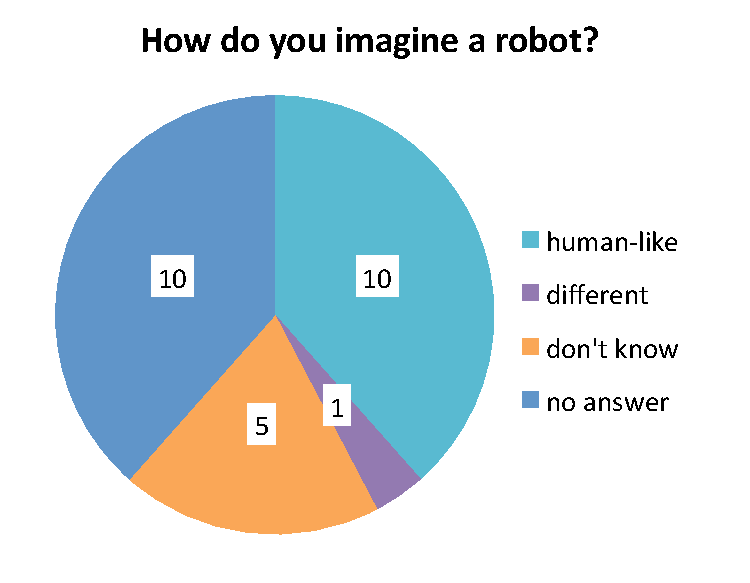
\includegraphics[width=4.75cm]{domino-imagine.pdf}
    }
    %    \hspace{0.2cm}
    \subfloat[] {
        \label{fig:domino-robot}
        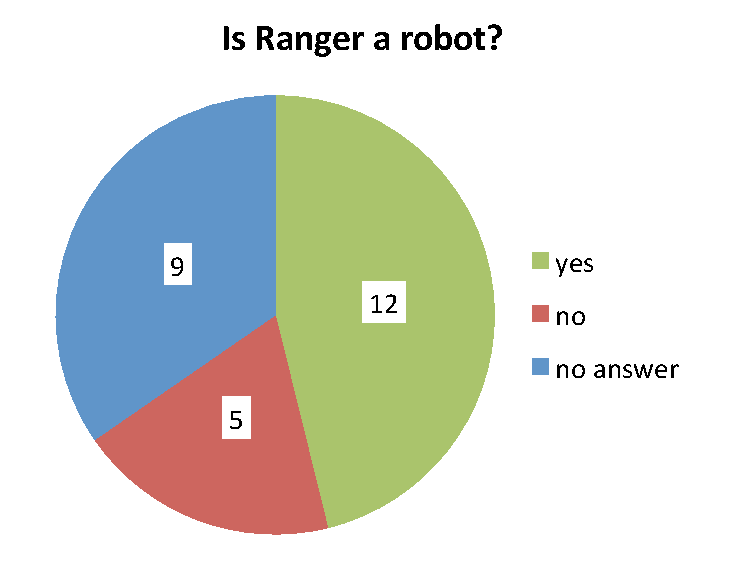
\includegraphics[width=4.75cm]{domino-robot.pdf}
    }
    %	\hspace{0.2cm}
    \subfloat[]	{
        \label{fig:domino-ranger-how}
        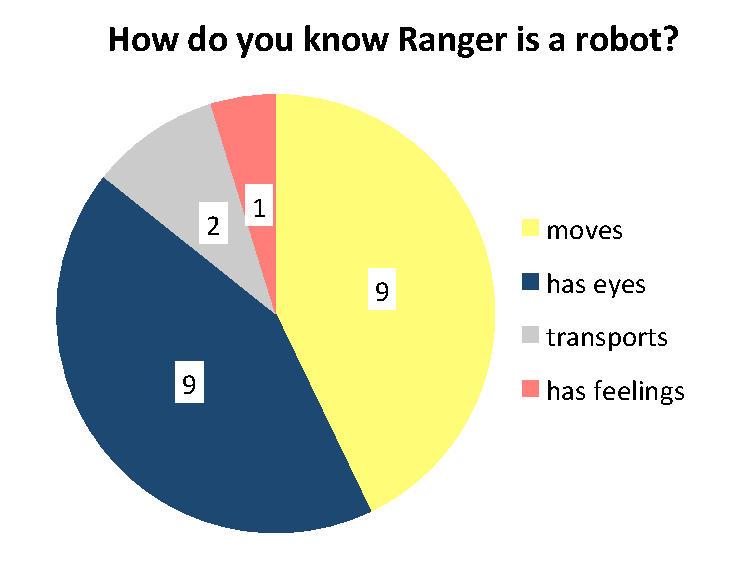
\includegraphics[width=4.75cm]{domino-ranger-how.pdf}
    }
    \caption[Expectations and Robot-likeness or Ranger]{\small
    \textbf{Expectations of robots in general and robot-likeness of Ranger.}
    When children had to justify why they thought Ranger is a robot (c), multiple
    answers were possible, we received 21 answers from 12 children.} 

    \label{fig:domino-expectations}
\end{figure}

\paragraph{First impression of Ranger}

Asked whether Ranger was a robot (see Figure~\ref{fig:domino-robot}), children
were not sure how to reply, and some hesitated or did not provide an answer at
all. In general, it was not easy for children to decide whether Ranger was a
robot or not because only a few of them had a clear concept of a robot in mind.
9 children did not give an answer at all. Some children mentioned they had had
different expectations (those who had a human-like image of a robot). From those
who replied, 5 children did not find that Ranger is a robot because it has no
arms or legs and because its eyes are not real. However the majority of the
respondents (12 of 17) was convinced of the opposite, namely that Ranger is a
robot. According to them (see Figure~\ref{fig:domino-ranger-how}) Ranger is a
robot because it is able to move by itself, it has eyes, it is able to transport
things, and because it has feelings (expressed by the light and sound cues).

\paragraph{Manipulation check} 

Before going into details about differences in the perception of the robot due
to the different misbehaviors, we need to check whether children noticed the
manipulations of the robot behavior, and how they interpreted them. Did they
perceive and classify the different misbehaviors, \textit{mistake, lost} and
\textit{disobey}, as we intended?  As stated in the beginning of the chapter, we
had hypothesized that the \textit{disobey} behavior is perceived as the robot
intentionally not doing what it should do. The \textit{mistake} behavior was
intended to show that the robot can do a mistake but is aware of it and able to
repair its mistake, which should also lead to some perception of intentionality.
Contrary, we expected that the \textit{lost} condition is perceived as a
malfunction or bug of the robot.  In the second interview, after the robot had
misbehaved, we asked children whether the robot always did what they wanted it
to do. Most children disagreed and said they noticed something strange. However,
there were some children who gave a positive answer, suggesting that they found
the robot always did what they wanted it to do. This was a surprise. Had they
not noticed the robot's misbehavior? Why not? On one hand, we found that
children sometimes gave contradictory replies when asked the same question
twice. This is difficult to interpret. On the other hand, children may have a
general tendency to please adults \cite{leite_long-term_2013}, and it could be
the case that some were too shy to tell us that the robot did something strange.

\begin{figure}[!h]
    \centering
    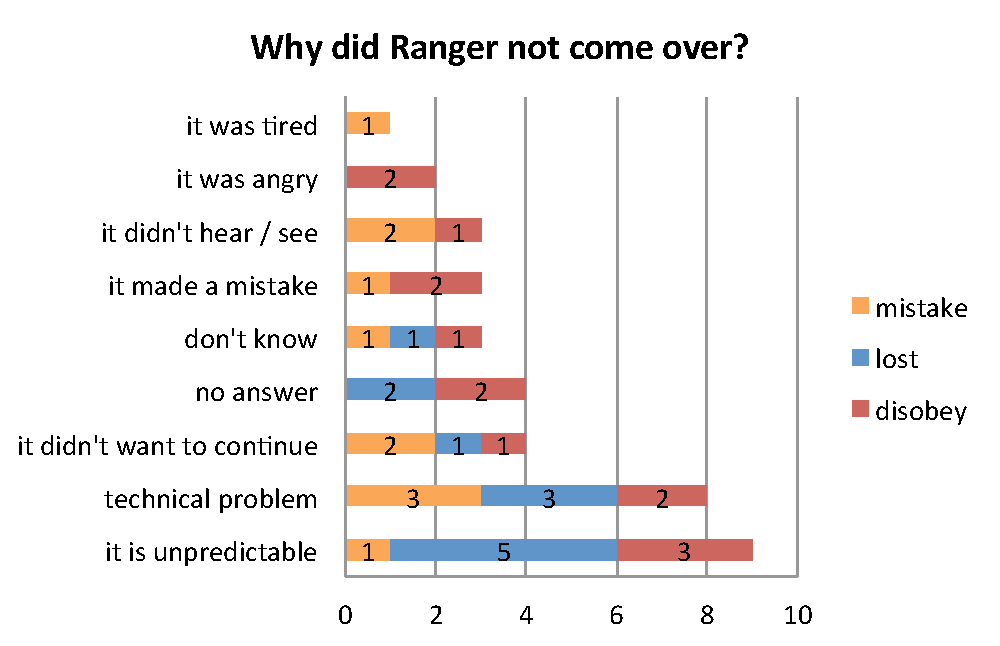
\includegraphics[height=6cm]{domino-why-misbehavior.pdf}   
    \caption[Why Did the Robot Misbehave?]{\small Multiple answers were possible
    to the question why the robot did not come over, and we received 37 answers.
    This question shows that children did not necessarily interpret the misbehavior
    in the way we had assumed.}

    \label{fig:domino-why-misbehavior}
\end{figure}	

We nevertheless asked children why they thought the robot had not always come
over to them. 4 of the children did not reply. The remaining ones gave a variety
of reasons (Figure~\ref{fig:domino-why-misbehavior}). The most common answer (9
of 37 replies) was that the robot is somehow \textit{unpredictable} in what it
is doing and that it could go \textit{no matter where}\footnote{We translated
children's answers from French to English. For some expressions the meaning and
connotation of an expression may not be the same. We understand \textit{``partir
dans tous les senses''} as ``to go off in all possible directions'' and hence
interpret this reflects viewing the robot as being unpredictable.} because
\textit{``with robots you have these kind of problems, they do no matter what''}
(boy (5), \texttt{lost4}). 8 replies concerned \textit{technical problems}
(including \textit{broken parts}), suggesting that children perceived the
misbehavior as unintended by the robot. 2 of the children who had interacted
with the disobeying robot said Ranger was \textit{angry}, which none of the
children in other conditions replied (these were not the two boys who reacted
aggressively). Several children ascribed intentionality to Ranger explaining
that it \textit{did not want to continue} carrying domino tiles or that it
\textit{made a mistake / did something silly}\footnote{We understood
\textit{``faire une bêtise''} as ``to do a silly thing'' in the sense of making
a mistake.}.

%\hl{(put some more quotes of the children, maybe even in French)}	

Overall, we can notice that not all children perceived the misbehavior of the
robot as we had intended and we have to keep this in mind while interpreting the
data. Also \cite{leite_long-term_2013} found in her study that when children did
not understand an action of the robot, they tended to view it as a mistake,
rather than interpreting the robot's behavior as a deliberative action.

%	\textit{``the supportive behavior ``Play Bad Move'' was not completely
%	understood as a deliberative action of the robot, but rather as a
%	mistake''}. 	

In our case, it is not easy to make a clear statement about how each of the
manipulations was perceived by the children.  Similar to how people reacted to
the cheating robot in the study of \cite{short_no_2010}, most children showed
surprise, were amused, sometimes confused, or occasionally slightly angry (\eg
two boys tended to shout to the robot after it had disobeyed). The
\textit{disobeying} robot seemed to evoke the strongest reactions, partly with a
negative implication: later three of the children in this condition stated they
would not accept Ranger as a friend \textit{because it did not always come over
when they asked it to come over}. \cite{short_no_2010} described a similar
implication of the robot cheating behavior: participants made unfavorable
character attributions to the cheating robot, so the robot's actions affected
perceptions of the robot as ``fair'' and ``honest''.


%	\cite{short_no_2010} found that participants often had an emotional reaction
%	to the robot's behavior and made unfavorable character attributions to the
%	cheating robot. The robot's actions affected perceptions of the robot as
%	``fair'' and ``honest''. Qualitatively, the authors found that participants'
%	reactions in the verbal cheat case tended more towards confusion, while
%	their reactions to the action cheat were more exaggerated, showing surprise,
%	amusement, and occasionally anger.  	

%	\cite{short_no_2010} found that participants who saw the action cheat
%	mentioned cheating, while the participants who saw the verbal cheat
%	frequently described it as a mistake or malfunction, while only sometimes
%	calling it cheating.

\begin{figure}[!h]
    \centering
    \subfloat[]{
        \label{fig:domino-hear}
        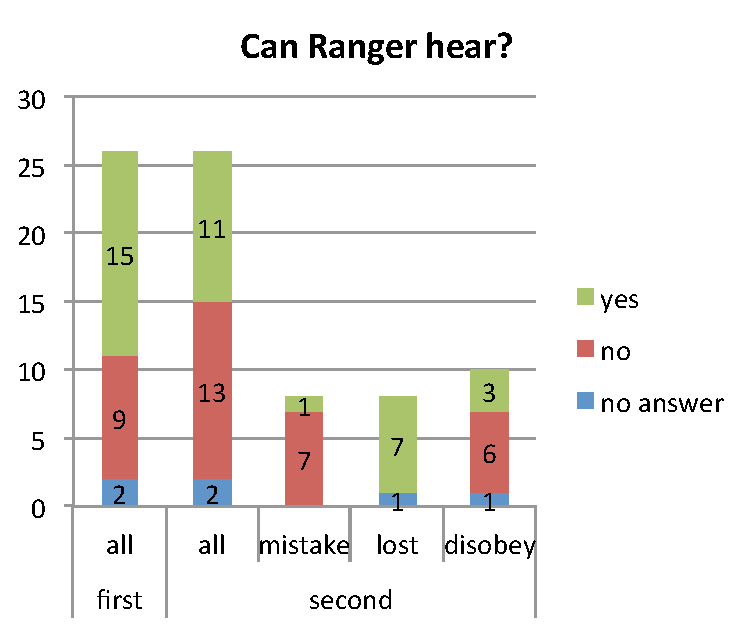
\includegraphics[height=5.5cm]{domino-hear.pdf}
    }
    \subfloat[] {
        \label{fig:domino-see}
        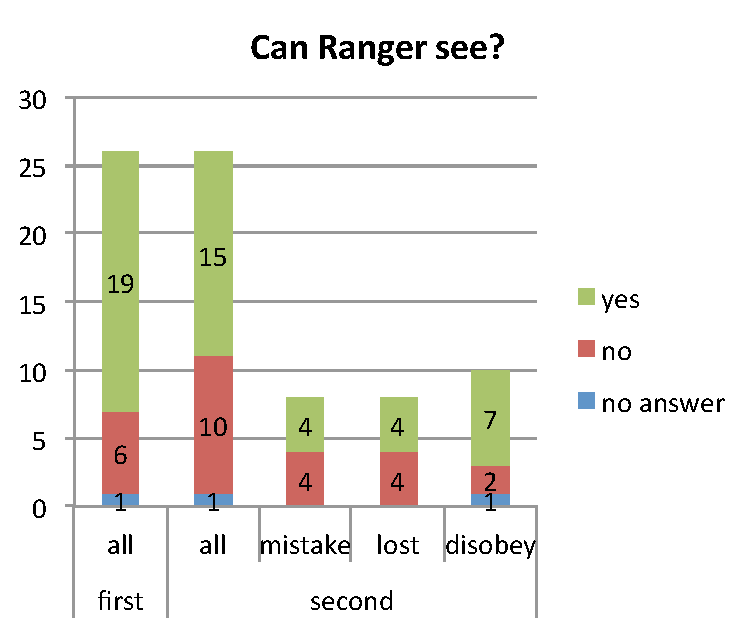
\includegraphics[height=5.5cm]{domino-see.pdf}
    }
    \caption[Attribution of Cognitive Skills to Ranger]{\small
    \textbf{Attribution of cognitive skills to Ranger.} These two questions were
    asked both in the first interview, after children had interacted with the
    correctly behaving robot, and in the second interview, after children had
    interacted with the unexpectedly behaving robot (three conditions). A comparison
    of the answers (first-second) can reveal to what extent the respective
    misbehavior of the robot impacted children's attribution of cognitive abilities.
    (Note that there were 10 participants in the disobey condition and each 8
    participants in the mistake and lost condition. Consequently, here and in the
    following visualizations, we need to be careful as the bars are based on
    counting answers.) The three bars on the right side of each diagram are a
    split-up of the \textit{``all''} bar of the second time children were asked.}
        
    \label{fig:domino-cognition}
\end{figure}	 
 
\paragraph{Attributions of cognitive abilities (perceptual skills)}

To assess how far children ascribed low-level cognitive abilities to the robot,
we asked them whether they believed Ranger is able to hear and see
(Figure~\ref{fig:domino-cognition}). Also these questions were asked both in the
first and the second interview. First, the majority of children replied
positively, saying that Ranger can hear (15) and can see (19). We asked them to
justify their answer in both cases (\textit{``How do you know?''}). Those
ascribing cognitive abilities answered, for instance: \textit{``It can see
because it is looking right at me.''} (girl (4), \texttt{disobey4}) or
\textit{``The only thing it can hear is when you say `come here'.''} (boy (5),
\texttt{mistake2}). Those who answered negatively added, for instance:
\textit{``It cannot see because the eyes are not real.''} (girl (4.5),
\texttt{disobey1}); \textit{``It cannot hear because it doesn't have ears.''}
(boy (4), \texttt{mistake4}); and surprisingly two 4-year old children mentioned
that Ranger is not able to hear because it does not have a \textit{mouth}. It
seems that for some younger children the concepts of speaking and hearing are
both related to a mouth. From those two questions, we can summarize that after
children had interacted with the \textbf{correctly behaving robot} the majority
does \textbf{ascribe cognitive abilities} to the robot.\\

After they had interacted with the misbehaving robot, some children responded
differently. Now 11 children (first 15) answered Ranger can hear, and 15
children (first 19) responded it can see. 2 children in the \textit{mistake}
condition consistently changed their opinion for both hearing and seeing
abilities. The other changes were not consistent for both senses and partly even
contradicting. There was no clear tendency, and also we cannot say whether the
different conditions had a different impact. We can note that also to the
\textbf{unexpectedly behaving robot} children tend to \textbf{ascribe cognitive
abilities} but slightly less than before. It seems that initially the
attribution of cognitive abilities is due to the robot's physical design (\eg
eyes) and that the manipulation of the robot's behavior does not substantially
change this perception (only for few children). 


\begin{figure}[h]
    \centering
    \subfloat[] {
        \label{fig:domino-obey}
        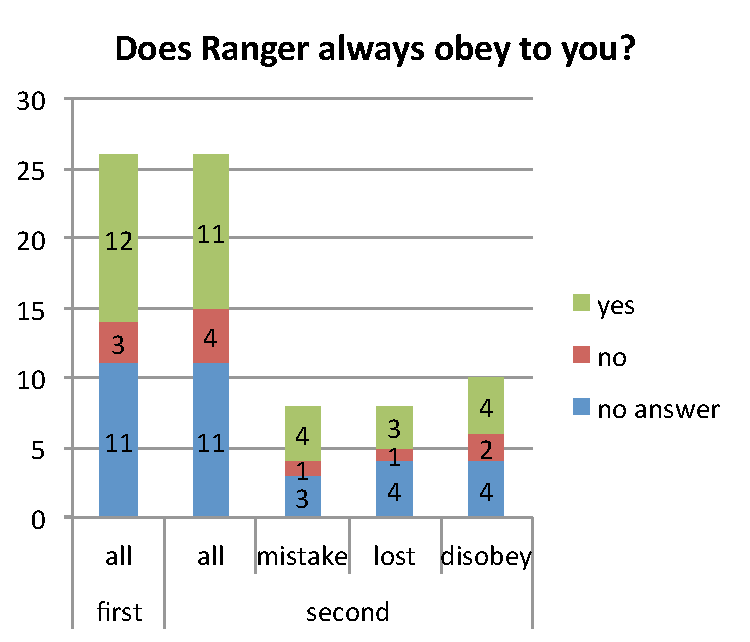
\includegraphics[height=5.8cm]{domino-obey.pdf}
    }
    \subfloat[] {
        \label{fig:domino-silly}
        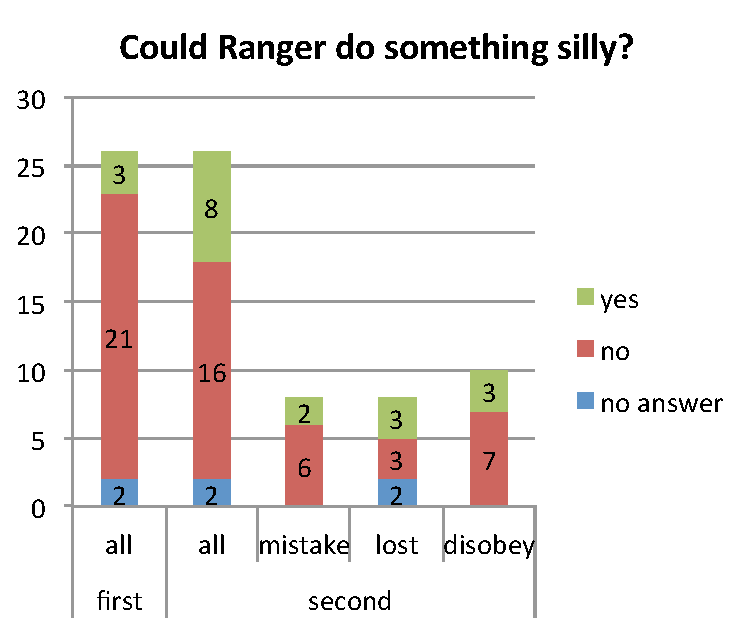
\includegraphics[height=5.8cm]{domino-silly.pdf}
    }
    \caption[Attribution of Intention to Ranger]{\small \textbf{Attribution of
    intention to Ranger.} Similar as before, children were asked these questions
    twice. Concerning question (a), there are no remarkable differences in
    children's responses given in the \textit{first} and \textit{second} interview.
    Children tend to think Ranger does always obey to them, even after it misbehaved
    (\textit{second} part). There is however a small difference in the responses
    visualized in graph (b). After the robot misbehaved, 8 children think the robot
    could do something silly whereas first, only 3 children answered like this.}
    
    \label{fig:domino-intention}
\end{figure}		

\paragraph{Attributions of intention}

One of the central points of this study was to investigate to what degree
children attribute intention and cognitive abilities to the robot.  In the first
interview after children had interacted with the correctly behaving robot we
asked three questions to assess how far they ascribe \textbf{intention} to it
(see questionnaire items in Table~\ref{tab:domino-questions},
page~\pageref{tab:domino-questions}). One of these questions was whether they
believed Ranger could go out the door by itself. They majority of 16 children
answered negatively, which suggests that they initially do not ascribe intention
to the robot. The two other questions were whether Ranger would always obey and
whether Ranger could do a silly thing (Figure~\ref{fig:domino-intention}). These
two questions were asked again later after children had interacted with the
unexpectedly behaving robot.

%	With these recurring questions we wanted to see whether children had changed
%	their mind in terms of ascribing intention to Ranger (and whether the
%	unexpected robot behavior had caused this effect). This comparison turned
%	out to be difficult, however.  	

Overall, in the first interview 12 of the 26 children believed Ranger does
always obey to them. Asked whether Ranger could do something silly, the great
majority of 21 children replied negatively. We can summarize that after children
had interacted with the \textbf{correctly behaving robot} the majority does
\textbf{not ascribe intention} to the robot.

After they had interacted with the misbehaving robot, we asked children again.
Now, still 11 children (previously 12) believed Ranger would always obey to
them. When analyzing the answers of each child separately, there were 2 children
in the \textit{disobey} condition that changed their answer from \textit{yes} to
\textit{no}; however also 1 child in the \textit{lost} condition that switched
their answer in the opposite way (strangely). There was a more remarkable change
when asking children whether Ranger could do something silly. In the second
interview, 8 children (previously~3) answered Ranger could do something silly. 1
child in the \textit{disobey} condition had changed their answer, and each 2 in
the \textit{mistake} and \textit{lost} condition. 

Overall, it it interesting to note that children tend to ascribe cognitive
abilities to the robot, like the ability to see and hear but not intention. We
interpret that children may perceive the robot as being able to process sensory
information but that it is not able to make decisions on its own. We can
summarize that even with the \textbf{unexpectedly behaving robot} children do
\textbf{not necessarily ascribe intention} to the robot. The unexpected robot
behavior impacted only some children's attributions of intention to the robot.
It seemed that some children did not interpret the robot's misbehavior as
intentional but more like a technical problem or mistake. For instance, even
after the robot misbehaved by \textit{disobeying}, the majority of the children
in this condition was still convinced that the robot could not do a silly thing
(Figure~\ref{fig:domino-silly}).


\paragraph{Attributions of emotional state and perceived companionship}

We examined whether children attributed \textbf{feelings} to the robot by asking
them (once at the end of the experiment) if they thought that Ranger can feel
happy or sad sometimes (Figure~\ref{fig:domino-feelings}). The great majority of
children (21 of 26) gave a positive answer. Only 2 children who had interacted
with the \textit{disobeying} robot did not believe that Ranger has feelings and
another 3 children (2 \textit{disobey} and 1 \textit{lost}) did not reply at
all. Overall, data suggests that \textbf{children attributed emotional states}
to the robot. Asked for more details, several children answered that it is
through its colors and sounds that the robot shows a feeling. Most children said
that they could make the robot feel happy by playing with it and putting a
domino tile inside the box. This may also be a reflection of their own feelings,
projected on the robot.  More than half of the children (14 of 26) agreed Ranger
can be their friend. We did not ask about what being a friend means to them but
as children generally liked playing with the robot, this may be linked to each
other. We can note that children \textbf{ascribe feelings to the robot and
partly accept that it can be a ``friend''}.

\begin{figure}[!h]
    \centering
    \subfloat[]
    {   \label{fig:domino-feelings}
        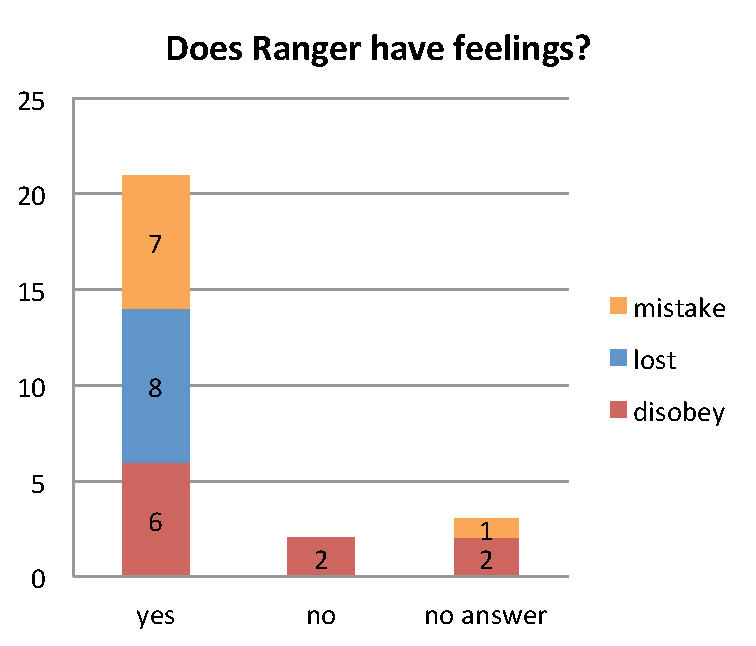
\includegraphics[height=5cm]{domino-feelings.pdf}}
    \subfloat[]
    {   \label{fig:domino-friend}
        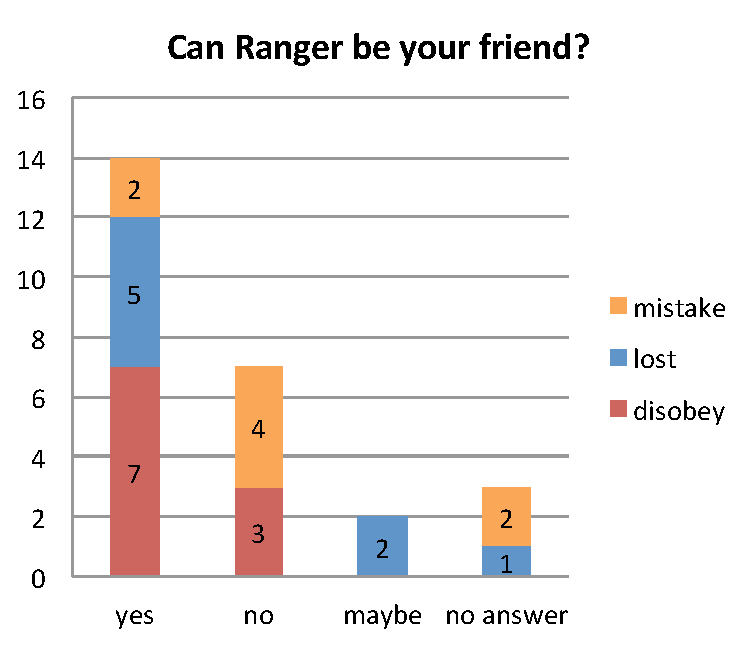
\includegraphics[height=5cm]{domino-friend.pdf}}
    \caption[Attribution of Emotional State and Perceived Companionship]{\small
    \textbf{Attributions of emotional state and perceived companionship}.}

    \label{fig:domino-feelings-companion}
\end{figure}

\paragraph{Attributions of moral standing}

Inspired from the questionnaire used by \cite{kahn_jr._robotic_2006}, we asked
children if it would be alright to leave Ranger alone at home (\eg during two
weeks when they go on a vacation) (Figure~\ref{fig:domino-leave}). The great
majority of 20 children responded negatively. Asked why, children gave a variety
of answers that we classified into 7 categories
(Figure~\ref{fig:domino-leave-why}). With 5 replies, the most common answer was
that the robot ``could do something silly''. Some other children simply answered
they would like to take it with them. Others were afraid that the Ranger ``would
not find its way'' or ``may be taken away by someone''. 2 children believed
Ranger is sad when left alone and 1 child responded the robot would try to
escape. This shows that some children really ascribed emotions or an ``own
will'' to the robot.  We can summarize that children generally \textbf{ascribe
moral standing to the robot}, meaning that it is an entity that deserves some
kind of respect and care. 

\begin{figure}[!h]
    \centering 
    \subfloat[] {
        \label{fig:domino-leave}
        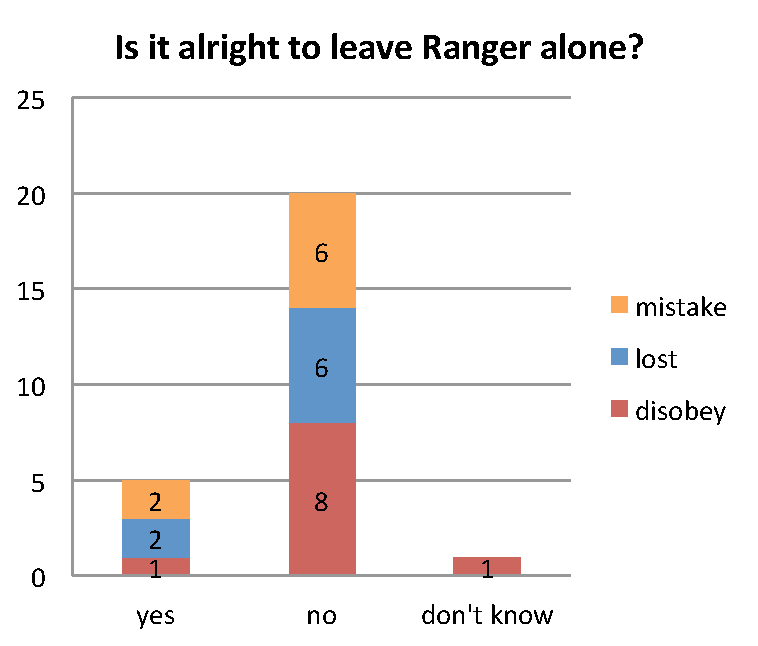
\includegraphics[height=5cm]{domino-leave.pdf}
    } 
    \subfloat[] {
        \label{fig:domino-leave-why}
        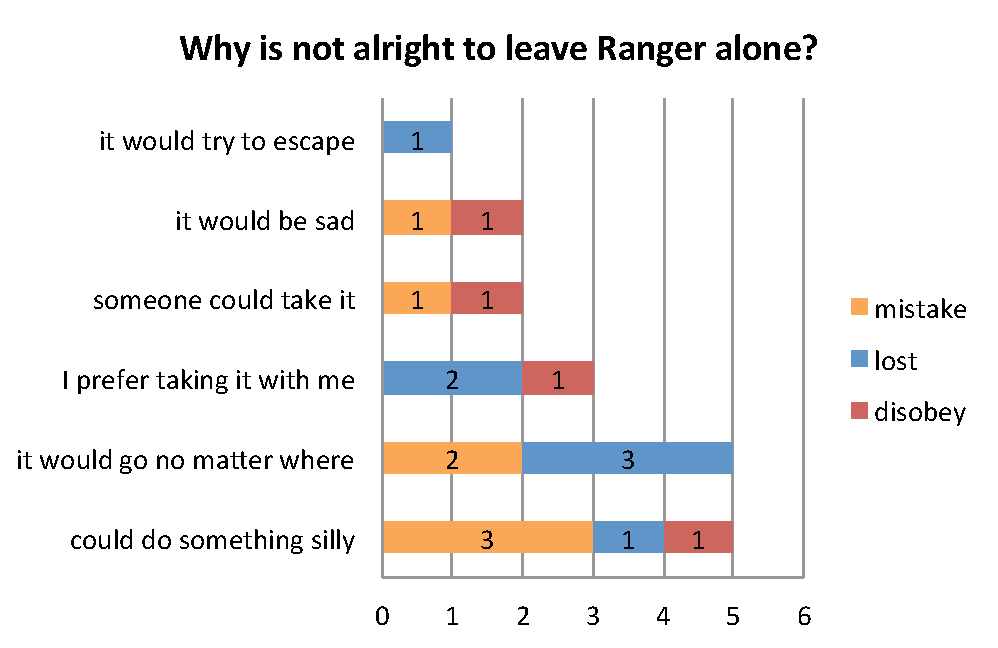
\includegraphics[height=5cm]{domino-leave-why.pdf}
    } 
    \caption[Attribution of Moral Standing]{\small \textbf{Attributions of moral
        standing}. We asked children whether it was alright to leave Ranger
        alone at home if they go on a 2-week vacation (a). Multiple answers
        (open-ended) were allowed when asked to justify their answer (b).}

    \label{fig:domino-leave-alone} 
\end{figure}		

\paragraph{Acceptance of Ranger}

It does not come as a surprise that children showed great fascination for the
robot and the domino game (we cannot clearly separate these two things). Only
those children whose expectations of the robot were not met, seemed to be
skeptical. Asked if they like Ranger, 16 children gave a positive reply and
there was no negative response, however 10 children did not answer this
question. Also, 18 of the children answered they would like to have Ranger at
home. Still 5 children gave a negative reply and 3 did not provide an answer at
all. 

\begin{figure}[!h]
\centering
 \subfloat[]
  {\label{fig:domino-like}
  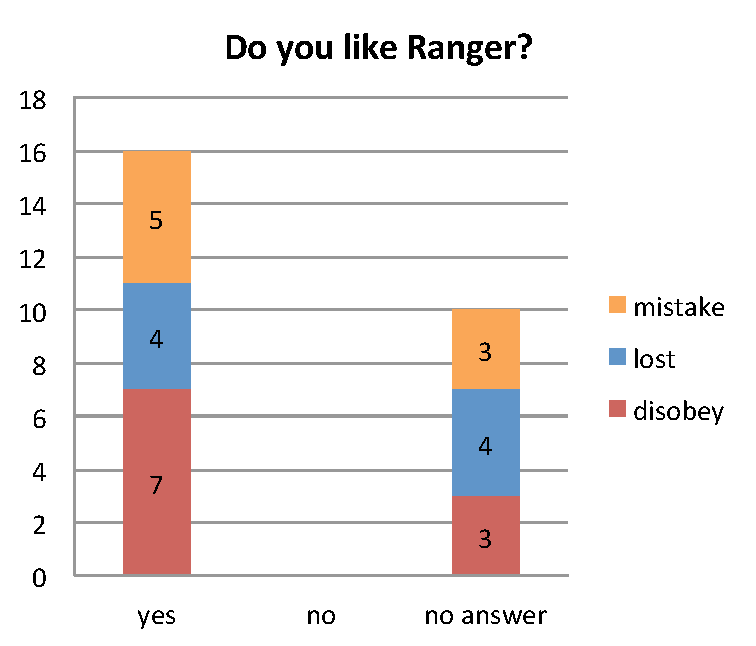
\includegraphics[height=5cm]{domino-like.pdf}}
 \subfloat[]
  {\label{fig:domino-leave-athome}
  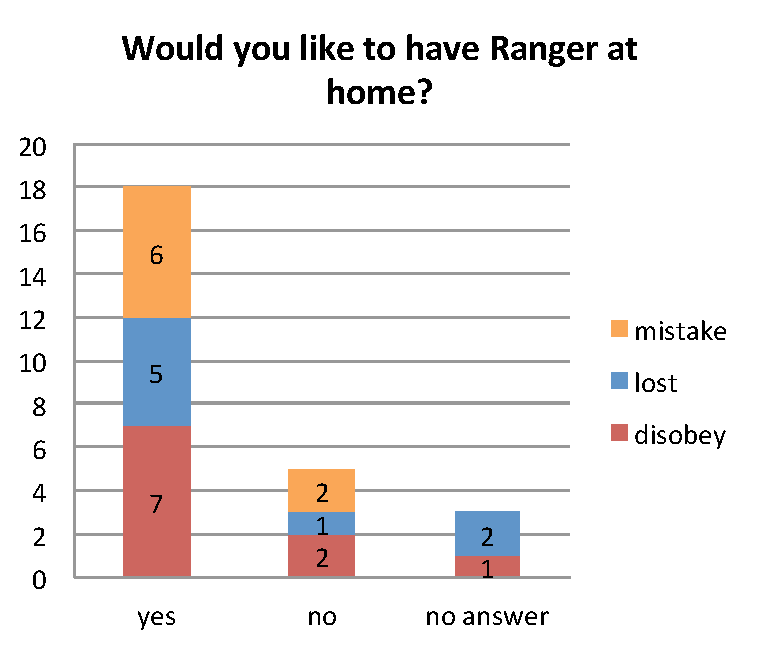
\includegraphics[height=5cm]{domino-athome.pdf}}
\caption[Acceptance of Ranger]{\small \textbf{Acceptance of Ranger}.}
  \label{fig:domino-acceptance}
\end{figure}
   


\paragraph{Summary}

In general, children tended to associate a robot with some human-like design and
characteristics, and they were hence not sure whether Ranger counts as a robot.
According to the children, Ranger's ability to move and its moving eyes however
suggest it is a robot.

Their perception of Ranger shows that they commonly ascribed some human-like
characteristics to the robot, such as emotional states or cognitive abilities,
and that they also tend to view it as a social entity (\eg by ascribing moral
standing, and accepting it as a friend). But children do not necessarily ascribe
intention and own reasoning to the robot. This suggests that anthropomorphism is
not something discrete being either \textit{there} or \textit{not there}; it may
rather exist in several variations or levels. (We explore social engagement and
anthropomorphism in more detail in the next section and come back to it in the
Conclusions Chapter of this thesis.) 

Concerning the manipulation of the robot behavior, most (but not all) children
recognized something strange and agreed that the robot did \textit{``no matter
what''}. The different types of misbehavior were not clearly interpreted as we
had intended. The robot's behavior was mostly perceived as
\textit{``unpredictable''}. Qualitatively, it seemed that the
\textit{disobeying} robot had a stronger impact on children's perception of the
robot than the other two behaviors \textit{mistake} and \textit{lost}.
Generally, children like Ranger and most said that they would like to play with
it at home.\\


%Also \cite{leite_long-term_2013} reported that when the iCat (the robot used in
%the study) said something that children were not expecting, the most salient
%affective expression was surprise.  6 out of the 16 children who took part in
%the study talked to the robot from the first until the last week of
%interaction. The most frequent words that children said to the robot were
%``thank you''. (we also observed this in the Domino Study)

\subsection{Anthropomorphism Index and Social Engagement with Ranger}

The anthropomorphism index expresses to what extent children engaged with Ranger
in a human-like way, both in terms of their behavior toward the robot and their
perception of the robot. We mostly present findings on a pair (group) level but
also look at differences between children in one group. 

As described in Section \ref{sec:domino-anth-score}
(page~\pageref{sec:domino-anth-score}), the anthropomorphism index considers on
one hand whether children behaved toward the robot in a human-like way. The
behavioral aspects refer to a qualitative analysis of the interaction, and not
to the counts of actions annotated in the video material. These qualitative
aspects included use of direct speech toward the robot, use of social pointing
gestures (\eg waving or nodding), and use of polite formulations. For instance,
several children said \textit{``thank you''} when Ranger brought a domino tile
to them or used a polite formulation when calling Ranger: \textit{``Robot,
please come over!''}\footnote{These forms of politeness that children use when
talking to a robot have also been observed by \cite{leite_long-term_2013}.}. If
a child was using such formulations, he or she was assigned 1 point, and at the
end, the sum of these points formed the anthropomorphism index. On the other
hand, the anthropomorphism index considers to what degree children perceive the
robot as human-like. These results have been mostly presented in the previous
section (\eg attribution of feelings to the robot). 

To obtain the anthropomorphism index for a pair, we first calculated the index
per child and then took the average of the two children in one group.  The group
indexes varied between 3.25 and 10.75 points with an average of 7.5 points
(SD~=~2.5), which is 47~\% of the maximum possible index of 16 points. Similar
to the individually different interaction styles of the children, there were
also variations in terms of to what extent they anthropmorphized Ranger. In 7 of
the 13 groups, the anthropomorphism indexes for both children were similar
(difference less than 1.5 points), which means that both children
anthropomorphized the robot to a similar degree. This agreement among children
happened for both higher and lower indexes. In 6 of the 13 groups, the
anthropomorphism indexes varied in more than 2 points, which means that one of
the children anthropomorphized the robot more than the other one. This is an
interesting finding.

On an overall average, Ranger was moderately anthropomorphized by the
children.\footnote{However, as our developed anthropomorphism score is relative,
we cannot really make a claim about what a difference of \textit{+} or \textit{-
1} point means.} 8 of the 13 groups had an index of 8 or higher.
Table~\ref{tab:domino-anth-score} shows that of those groups, 3 were in the
\textit{mistake} condition, 3 in the \textit{lost} condition and 2 in the
\textit{disobey} condition. Also, the mean index of anthropomorphism in the
three conditions varied, with the \textit{mistake} and \textit{lost} condition
leading to a higher index than the \textit{disobey} condition.	This finding
suggests that the disobeying robot was less anthropomorphized than the other two
robot behaviors, which speaks against our second hypothesis. We had expected
that the disobeying behavior is perceived as an intentional action which we
assumed would lead to increased anthropomorphism. This was not the case. The
slight difference between the \textit{lost} and \textit{mistake} robot was also
expected in the opposite direction. It could be that the robot's
``helplessness'' led to this. With the lost robot, children looked more often at
the experimenter than in the other condition (see
Table~\ref{tab:domino-conditions}, page~\pageref{tab:domino-conditions}), which
suggests that they could not fully make sense of the robot's behavior. The fact
of not being able to understand (and hence predict) a robot's behavior is likely
to increase anthropomorphism.\footnote{One of the cognitive / psychological
explanations for anthropomorphism is that people want to make sense of something
they do not understand and then tend to anthropomorphize this something (human
traits are a good source of making attributions because this is what people
understand best -- themselves and other humans). For more details the reader may
refer to \cite{epley_seeing_2007}.}

\begin{table}[ht!]
\label{tab:domino-anth-score}       % Give a unique label
\centering
\footnotesize
\begin{tabular}{lccc}
\noalign{\smallskip}\noalign{\smallskip}\hline\noalign{\smallskip}
	& \multirow{2}{*}{M} & \multirow{2}{*}{SD} & count of groups with \\ 
	& & & with index above 8 \\
\noalign{\smallskip}\hline\hline
	\textit{mistake} & 7.94 & 1.74 & 3 of 4 \\ 
	\textit{lost} & \textbf{8.31} & 0.59 & 3 of 4 \\ 
	\textit{disobey} & 6.5 & 3.68 & 2 of 5 \\
\noalign{\smallskip}\hline
\end{tabular}
\caption{\textbf{Anthropomorphism index.} The maximum possible index was 16. The \textit{lost} robot elicits the highest index, which suggests that it is anthropomorphized more. Contrary to our hypothesis, data suggests that the \textit{disobeying} robot is anthropomorphized less but the \textit{lost} robot more.}
\end{table}	

But to what extent is the human-like interaction related to perceiving the robot
as human-like? Do children who interact a lot and are probably more engaged with
the robot also perceive the robot as more human-like? This was what we
hypothesized. Data suggests the opposite, however. As shown in
Figure~\ref{fig:domino-anthropo-interaction}, we found a significant
\textit{negative} correlation between the count of engagement actions (per
group) and the qualitative anthropomorphism index (r(11)=-0.56, p=.05).

%	(b=-.05, t(11)=-2.22, p=.048). 

The overall model with the count of engagement actions (per group) predicts a
significant proportion of the qualitative anthropomorphism index (adjusted
R$^2$=.25, F(1,11)=4.9, p=.05). This means that the more a group showed
engagement in the interaction, the less they anthropomorphized the robot. This
is a key results, which was against our initial assumption. How can we interpret
this? It may be that children who interact more with the robot understand better
how it works, they are more familiar with it, and as such the robot appears less
``mystical'' to them, so there is not a big need to anthropomorphize it. On the
contrary, the cluster of groups that do not interact much but anthropomorphize
the robot more, is quite homogeneous. The negative correlation between the
number of engagement actions and the anthropomorphism index suggests that
children who interact more with the robot tend to anthropomorphize it less. This
implies that anthropomorphism could fade out after some time (or rather after
some interaction). This evokes the question how far anthropomorphism (as a
special kind of social engagement) really helps in sustaining interaction. This
is a critical point because most of the short-term investigations suggest that
anthropomorphic design and human social cues emitted by a robot foster
engagement and acceptance. What if this is not true for continued interaction,
and thus for the long-term?  We have to be careful about our interpretation, due
to the small sample size with which we obtained these findings. We suggest to
investigate the aspect further in future research.

\begin{figure}[t]
    \centering
    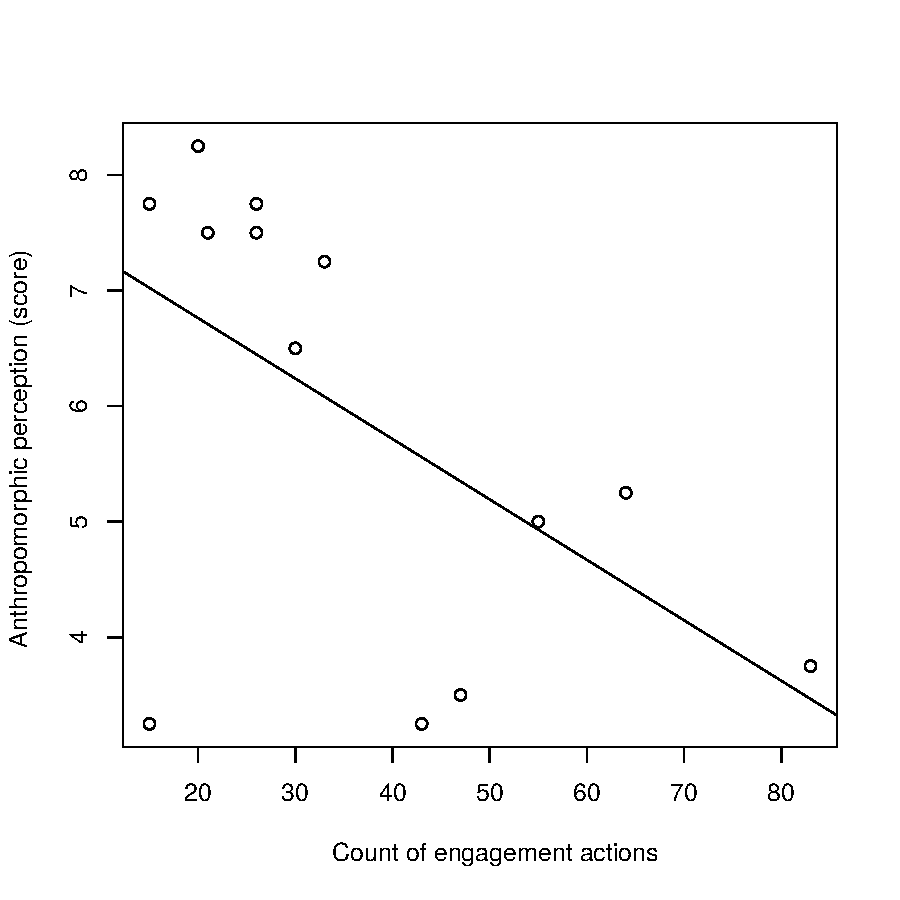
\includegraphics[width=0.8\columnwidth]{domino-correlation.pdf}   

    \caption[Correlation of Anthropomorphic Perception of the Robot and
    Interaction]{\small \textbf{Correlation of anthropomorphic perception of the
    robot and engagement actions.} A scatter plot of the count of engagement
    actions (without explore) and the \textit{anthropomorphic perception} (score per
    group) shows a negative correlation. The score for the anthropomorphic
    perception (\textit{y-axis}) does not take into account the behavioral aspect of
    the anthropomorphism index, as this is part of the interaction
    (\textit{x-axis}).  There seem to be two clusters of groups: those who interact
    more with the robot and anthropomorphize it less, and those who interact less
    but anthropomorphize the robot more.}

    \label{fig:domino-anthropo-interaction}
\end{figure}	

Our data on the anthropomorphism index also suggest \textbf{qualitative gender
differences} in children's tendency to anthropomorphize Ranger. Boys (M=8.2,
SD=3.0) obtained a higher mean index of anthropomorphism than girls (M=6.4,
SD=2.4). (Interestingly, as it was mentioned before, boys interacted slightly
more with the robot than girls; though not significantly. This is
counter-intuitive concerning the negative correlation between amount of
interaction with the robot and anthropomorphism tendency.) It would be
interesting to investigate in more detail whether boys are more prone to
anthropomophize a robot than girls.\footnote{Findings presented in
\cite{schermerhorn_robot_2008} suggested similar gender differences. In their
study, males tended to think of the robot as more human-like and accordingly
showed more ``social facilitation'' than females, who perceived the robot as
more machine-like.} 

%	\hl{(is this consistent with previous work?)}

\paragraph{Summary}

The established \textit{anthropomorphism index} suggests that children tend to
conditionally anthropomorphize the robot. Higher indexes of anthropomorphism
were found in the \textit{lost} and \textit{mistake} condition which was against
our hypothesis. Interestingly, data suggests a significant negative correlation
of engagement and anthropomorphism index. It appears that groups who interacted
more with the robot perceived it as less-humanlike. This raises the question to
what extent anthropomorphic perceptions of a robot can last over time, and with
increasing interaction experience.

\section{Discussion}

\subsection{Engagement and Anthropomorphism}


\section{Conclusions}

We found that in a playful scenario where 4-5 year old children play domino
together with a robot, the robot seems to be more engaging when it shows some
misbehavior compared to when it always behaves as expected.\footnote{However, we
cannot say if this effect holds also after novelty has worn off.} Different
types of misbehavior appear to have a different effect on children's interaction
and their perception of human-likeness in the robot. A \textit{disobeying} robot
may be perceived more negatively than a robot that makes a \textit{mistake} or
gets \textit{lost}. This may lead to attributions of negative personality to the
robot and children may be less motivated to continue interacting. Such effect
would be against our idea to promote long-term engagement. A similar conclusion
was drawn by \cite{short_no_2010}, in their study of a cheating robot:
Participants sympathized with a robot that \textit{verbally} cheated but they
behaved punitively towards a robot that cheated \textit{in its actions}.  Thus,
the effect depends on the type of misbehavior that the robot shows. With some
``lighter'' misbehavior, children may show helping-behavior and increase their
engagement, whereas using some ``stronger'' misbehavior, may lead children to
see the robot as being unpredictable and they could lose trust in it.

In general, any difference in robot behavior may have a strong effect on
children's perception of the robot, and can powerfully shape how they relate to
it: \textit{``The attribution of mental state to a robotic partner has dramatic
consequences for the relationship between robot and human. A friend has mental
state, a vacuum cleaner does not''} \cite[p.~225]{short_no_2010}.  From what we
have seen in the Domino Study, we have a rough estimate of how children react
and relate to a robot that behaves unexpectedly from time to time. They are
mostly surprised, laugh at the robot, and they tend to be more engaged and
playful. However, they are also confused and cannot really make sense of the
robot's strange behavior. We also cannot clearly say whether children perceived
the unexpected robot behavior entirely as a malfunction (something that happens
to a machine) or as being intended and based on a motivation (something related
to a social entity). Children stated both, when asked why the robot had
misbehaved. Some referred to \textit{``a technical problem''} while others said
the robot \textit{``is tired''} or it \textit{``doesn't want to carry domino
tiles any more but rather go on a tour outside''}. Maybe our manipulations were
not as clearly designed as we expected. There is always some freedom in how
things are interpreted -- especially with young children.  Certainly more work
needs to be done to investigate which robot behavior is most beneficial for
young children and can promote their engagement and motivation to interact with
Ranger over extended periods of time.  


%	Whereas a cheating opponent is acting out of a desire to win the game, a
%	malfunction, on the other hand, is entirely accidental, and could be the
%	fault of physical design or faulty programming, and can even occur entirely
%	without involvement on the part of the robot. \textit{``A malfunction is
%	something that happens to a machine, while a social entity that can cheat
%	has motivations and desires.'' Short et al.}


\subsection{Limitations}

This study and the results have several limitations.  First, we did not have a
real control group in which the robot always behaved correctly. Instead, we took
the first interaction phase as a reference for how children interact with the
correctly behaving robot.  Also, the sample size of 13 groups was small. There
were  variations in the data due to the individual differences of children. More
data could have allowed for a better comparison between the conditions.  With
the manipulation of the robot behavior we were able to surprise children.
However, it is questionable how often the same type of behavior manipulation
leads to surprise. Moreover, our experiment was a short-term interaction study
while we try to make statements about how to sustain long-term engagement. This
is critical but not unusual. Long-term HRI studies with young children are
extremely rare as they are difficult to set up as well as time and resource
consuming \cite{leite_long-term_2013}. Nevertheless, we could have probably
improved our study by setting up several short interaction sessions spreading
over several weeks. At the end of each session we could have asked whether
children want to play again with the robot. Such a study could have helped to
investigate the long-term interaction with the robot and the impact of the
behavioral variances.

\subsection{Lessons Learned}

One of the lessons learned is that it is difficult to set up a controlled lab
study with young children. Children are not like adults who patiently
participate in a 45-minutes experiment and then get some reward in the end. On
one hand, an experiment with children should not be boring for them, but on the
other hand, you would like to seriously collect some data. A lot of the
challenges we experienced are also described in \cite{ros_child-robot_2011}. One
of the most difficult parts turned out to be the interviews with the children.
We need to be careful to not over interpret some of their answers. Some children
seem to not have a clear opinion and partly contradict themselves. These answers
are not easy to interpret. An interview script including the questions need to
be designed very carefully, and should definitely be tested beforehand with the
respective age group.

Overall, it appears that when trying to study something in more detail, such as
the manipulation of robot behavior, 4-5 year old children may be too young. But
when trying to evaluate a more general approach, the design of a prototype, or
an interaction scenario, children are a very good choice. They say things as
they are and react very naturally, when compared to adults, who may reply more
socially desired. 


\paragraph{Summary}

In this study, we investigated the effect of unexpected robot behavior on
children's engagement in interacting with Ranger and on their perception of the
robot.  Our first hypothesis finds support: children show more engagement toward
a robot that behaves unexpectedly from time to time. Further, different types of
unexpected behavior may have a different effect, and therefore the behavior
manipulation needs to be designed with care.
We did not find support for our second hypothesis which stated that children
perceive a robot showing intention or cognitive abilities as more human-like
than a robot that appears to have a system error. This may be due to the study
setup and the fact that children did not interpret the robot misbehavior in the
conceived way. Our findings seem to suggest the contrary to our hypothesis. A
robot that appeared to do a \textit{mistake} or to be \textit{lost} was more
anthropomorphized than a robot that \textit{disobeyed}. But again, as children
may have misinterpreted these robot behaviors we cannot be sure about this
result.

Another outcome of this study is the initial development and first tryout of an
\textbf{anthropomorphism index}. This index considers both behavioral and
perception aspects and is able to indicate lower and higher levels of
anthropomorphism along this continuous index. At the moment, there is no such
index available that quantifies anthropomorphism along a scale and there is no
technique that combines behavior and perception. We may raise a discussion about
this in Chapter~\ref{chap:conclusion}.  In the future, we will need to refine
and improve this scale. For instance, we need to identify the specific factors
that should be included as measurement points in such a scale, for both aspects
(behavior and perception). Also, we need to think about how to balance the two
aspects appropriately. Probably, also characteristics of the person, the robot,
and the situation need to be considered. 

\nocite{johnson_detecting_2003}

\section*{Acknowledgments}

This research was supported by the Swiss National Science Foundation through the
National Centre of Competence in Research Robotics.

%%%%%%%%%%%%%%%%%%%%%%%%%%%%%%%%%%%%%%%%%%%%%%%%%%%%%%%%%%%%%%%%%%%%%%%%%%%%%%%%%%%%%%%%%%%%%%%%%%%%%%%%%%%%%%%%%%%%%%%%%%%%%%%%%%%%%
%%%%%%%%%%%%%%%%%%%%%%%%%%%%%%%%%%%%%%%%%%%%%%%%%%%%%%%%%%%%%%%%%%%%%%%%%%%%%%%%%%%%%%%%%%%%%%%%%%%%%%%%%%%%%%%%%%%%%%%%%%%%%%%%%%%%%
\bibliographystyle{abbrv}
\bibliography{domino}

\balancecolumns

\end{document}
